% =====================================================================
%  CHAPTER 4 — SYSTEM DESIGN
%  Section 4.1 (High Level Design) is in this file.
%  Section 4.2 (Low Level Design) is in parts/ch4b.tex, included at the
%  end of this file.
% =====================================================================
\clearpage
\chapter{System Design}

This chapter presents the design of the engine in two parts. Section~4.1
establishes the principle from which the architecture is derived, describes
the resulting structure, and justifies the decisions that the structure
encodes. Section~4.2 descends to the level of individual tables, queries,
transactions and goroutine handshakes, and includes the failure analysis that
determines what the engine can and cannot promise.

The chapter is written so that each mechanism is introduced by the problem it
solves. Where a design decision was contested, the rejected alternative is
stated along with the reason for rejecting it, because a design presented
without its alternatives cannot be assessed.

\section{High Level Design}

\subsection{The Governing Design Principle}

The entire architecture is derived from one invariant, stated here and
referred to throughout the remainder of the chapter as the governing
principle:

\begin{quote}
\textbf{Workflow code is a pure function of its event history.} Given the same
list of events, executing the workflow function produces the same sequence of
decisions, every time, on any machine.
\end{quote}

This is not a stylistic preference. It is the property that purchases every
capability the engine claims, and the relationship is worth making explicit.

\textbf{Crash recovery} requires no snapshot of memory, threads or stack
frames. The engine does not attempt to restore a process to the state it was
in; it re-executes the function against the saved history, and the stack
rebuilds itself as a side effect of that execution. A mechanism that saved and
restored memory would have to serialise closures, open connections and
goroutine stacks, none of which is portable between machines or across code
versions.

\textbf{Migration} between machines is free. A workflow can resume on a
completely different node because nothing machine-local was ever part of its
state. There is no affinity to re-establish and no cache to warm. This is what
makes shard failover a matter of ownership rather than of data movement.

\textbf{Debuggability} is structural rather than added. The history \emph{is}
the execution trace; there is no separate log to correlate against it, and no
possibility of the two disagreeing.

Everything else in this chapter is either machinery that keeps this principle
true, or machinery that keeps the history durable and available.

Two consequences constrain the programming model and are enforced rather than
merely documented. First, orchestration code may perform no input or output of
its own, because any value read from the environment --- the clock, a random
source, a file, a network response --- would differ between the original
execution and the replay, and would break determinism. Second, any unavoidable
non-determinism must be \emph{journalled}: executed once, its result written to
the log, and thereafter read from the log rather than recomputed.
Section~4.2.10 applies exactly this technique to the semantic deduplication
verdict, which is what makes that contribution defensible rather than ad hoc.

\subsection{Architectural Overview}

The system is organised into five tiers, shown in Fig.~\ref{fig:arch} and
summarised in Table~\ref{tab:tiers}. The tiers are logical rather than
physical: every node runs the whole stack above the persistence tier in a
single operating-system process.

\begin{figure}[htbp]
  \centering
  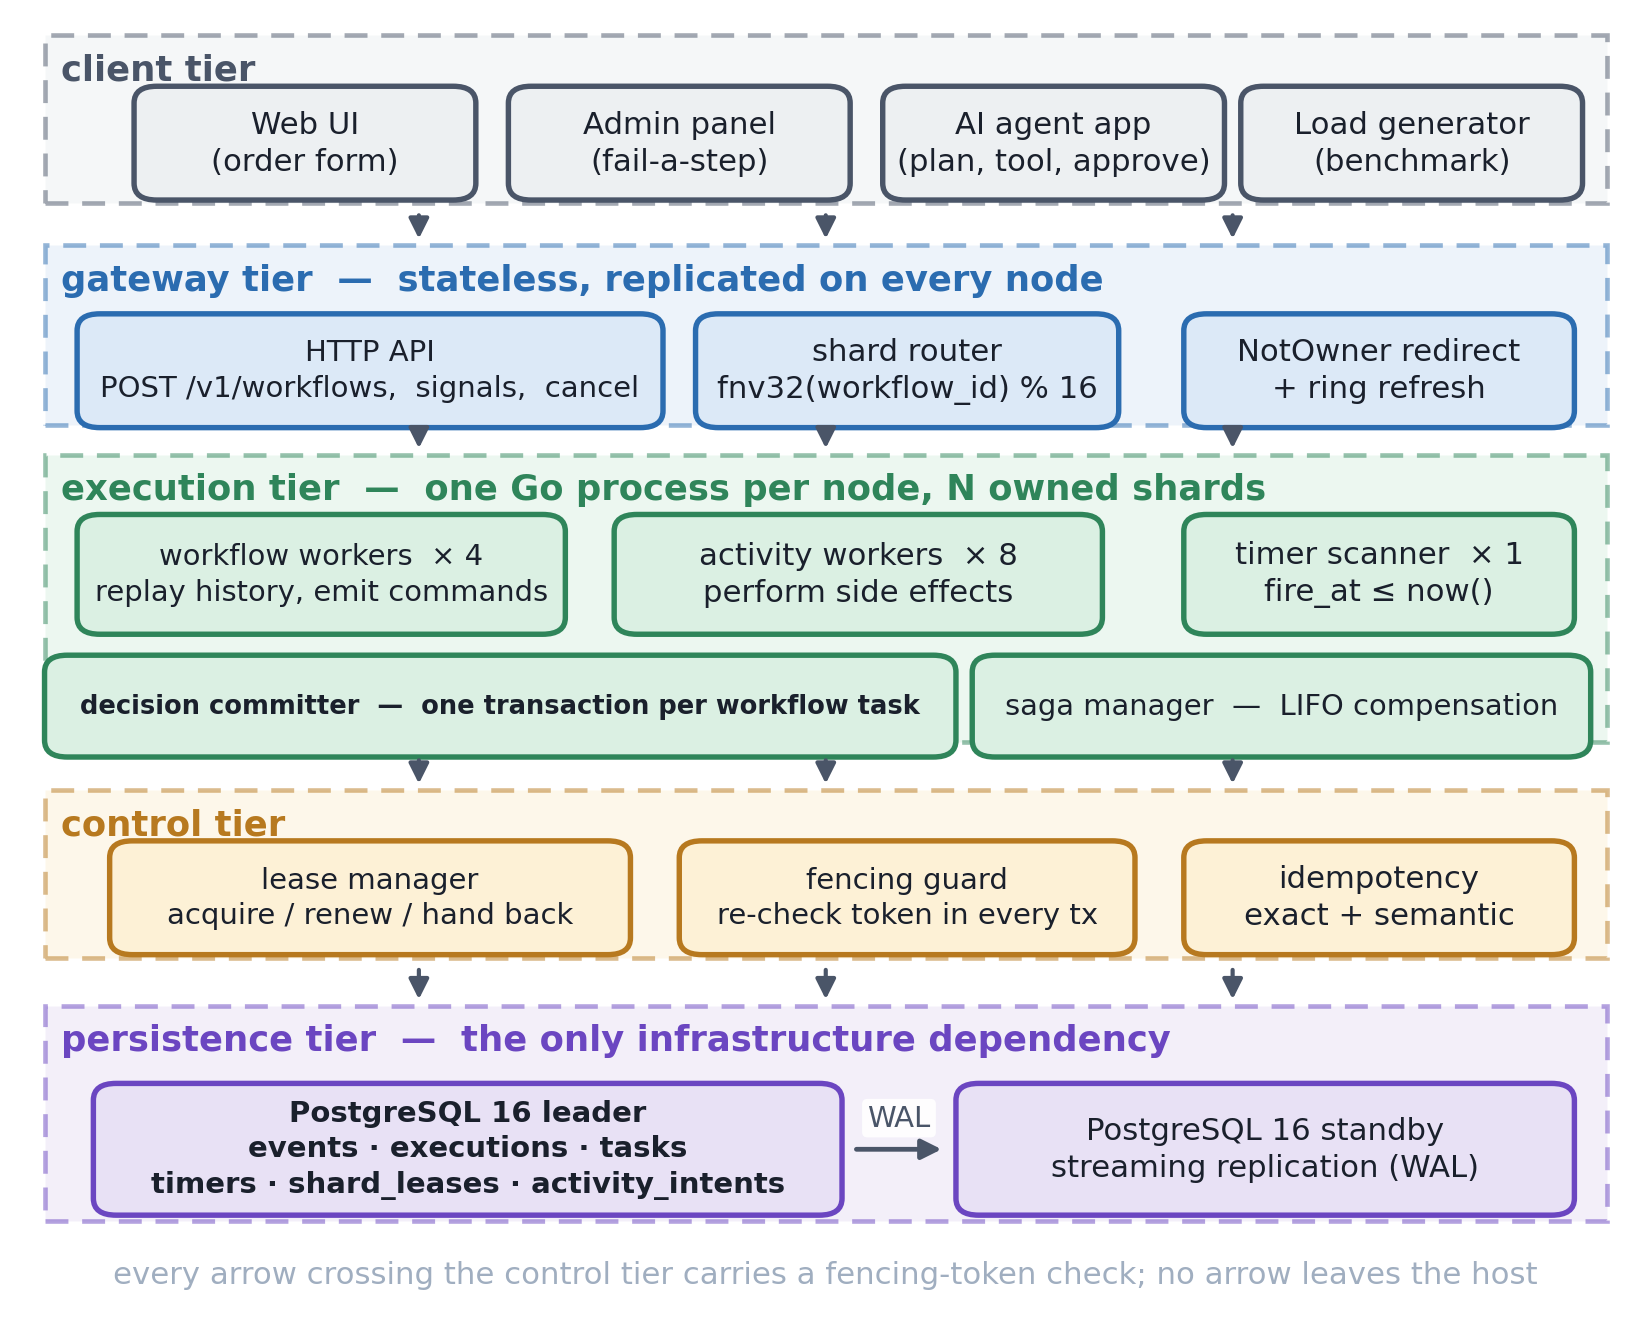
\includegraphics[width=\linewidth]{figures/fig_4_1_architecture.png}
  \caption{The five architectural tiers of the engine. Every node runs the
    client-facing gateway, the execution tier and the control tier in one
    process; only the persistence tier is shared. The control tier is where
    every mutating path is gated by a fencing-token check, which is what makes
    partitioned execution safe without a coordination service.}
  \label{fig:arch}
\end{figure}

\begin{table}[htbp]
  \centering
  \caption{Architectural tiers, their responsibilities and their state}
  \label{tab:tiers}
  \small
  \begin{tabular}{@{}p{0.75in}p{1.95in}p{1.85in}@{}}
    \toprule
    \textbf{Tier} & \textbf{Responsibility} & \textbf{State held} \\
    \midrule
    Client & Starts workflows, sends signals, observes progress, injects
      faults during evaluation & None \\
    Gateway & Routes a request to the node that owns the target shard;
      redirects when its routing view is stale & None. Deliberately stateless
      and replicated on every node \\
    Execution & Replays history, decides what happens next, performs side
      effects, fires timers, runs compensations & Only transient per-task
      state, discarded after every commit \\
    Control & Acquires and renews shard leases; verifies the fencing token
      inside every mutating transaction; evaluates idempotency &
      The fencing token currently held, in memory, re-verified on every write \\
    Persistence & Stores events, executions, tasks, timers, leases and
      activity intents; replicates to a standby & All durable state in the
      system, without exception \\
    \bottomrule
  \end{tabular}
\end{table}

Three properties of this structure are deliberate and are worth stating
separately.

\textbf{The gateway holds no state.} It hashes a workflow identifier, looks up
the owning node and forwards. If its view of ownership is stale it will
forward to a node that no longer owns the shard; that node replies with a
\cd{NotOwner} response naming the current owner, and the gateway refreshes and
retries. Routing is therefore allowed to be briefly wrong. Correctness is
enforced at the point of writing, not at the point of routing --- which is the
difference between a design that requires global agreement on a routing table
and one that does not.

\textbf{The execution tier keeps nothing between tasks.} When a workflow task
completes, the in-memory workflow state is discarded. Correctness never
depends on retaining it. Caching the workflow between tasks --- what Temporal
calls \emph{sticky execution} --- is a pure latency optimisation that can be
added and removed without any change in behaviour.

\textbf{The persistence tier is the only shared component}, and therefore the
only coordination point. This is the architecture's central trade-off, and it
is stated plainly in Section~4.1.7.

\subsection{The Separation of Workflow and Activity}

The programming model distinguishes two kinds of code, and the engine's
correctness depends on the distinction being maintained absolutely.

\begin{table}[htbp]
  \centering
  \caption{The contract between workflow code and activity code}
  \label{tab:wfact}
  \small
  \begin{tabular}{@{}p{0.7in}p{1.62in}p{1.08in}p{1.1in}@{}}
    \toprule
    & \textbf{Workflow} & \textbf{Activity} & \textbf{Enforced by} \\
    \midrule
    Decides & What happens next & Nothing &
      Review and the determinism detector \\
    Performs & No input or output whatsoever &
      All external side effects & Absence of I/O in the context object \\
    Determinism & Mandatory & Not required &
      Non-determinism error at replay (FR-3) \\
    Executions & Once per recovery, many times in total &
      At-least-once, ideally once & The replay mechanism \\
    Failure & Fails the workflow & Retried under policy &
      Retry policy on the activity \\
    \bottomrule
  \end{tabular}
\end{table}

The practical rule is that the workflow never does I/O and the activity never
makes orchestration decisions. Blurring the line does not produce an immediate
error; it produces intermittent non-determinism failures that appear long
afterwards and are extremely difficult to attribute. The engine therefore
makes the separation structural: the context object handed to workflow code
exposes no facility for performing I/O, so the ordinary way of writing the
code is also the correct way.

\subsection{The Two-Level Mapping: Workflows, Shards and Nodes}

Partitioning is expressed as two separate mappings, and keeping them separate
is the single most consequential decision in the architecture:
\[
  \texttt{workflow\_id}
  \;\xrightarrow[\;\text{\footnotesize $N$ fixed at deploy}\;]{\text{hash}}\;
  \texttt{shard\_id}
  \;\xrightarrow[\;\text{\footnotesize $\approx$150 virtual nodes}\;]{\text{consistent hash ring}}\;
  \texttt{node}
\]

The first mapping is $\texttt{shard\_id} = \mathrm{fnv32}(\texttt{workflow\_id})
\bmod N$, with $N$ fixed at deployment time and defaulting to sixteen. A
workflow never changes shard for the whole of its life. That permanence is
what makes its event log a stable, single-writer append stream, which in turn
is what allows the primary key alone to serve as the concurrency control
(Section~4.2.1).

The second mapping assigns shards to nodes through a consistent hash ring with
approximately one hundred and fifty virtual nodes per physical node. Adding or
removing a node moves a minority of shards and leaves every other shard
untouched.

Fig.~\ref{fig:mapping} shows why the indirection matters. Had workflow
identifiers been hashed directly to nodes, adding a node would move individual
\emph{workflows} between logs while they were still running, which is a data
migration performed under load on live state. With the fixed intermediate
mapping, adding a node moves only the \emph{right to act on} a shard. No event
is copied, no workflow is rewritten, and the operation reduces to a lease
changing hands.

\begin{figure}[htbp]
  \centering
  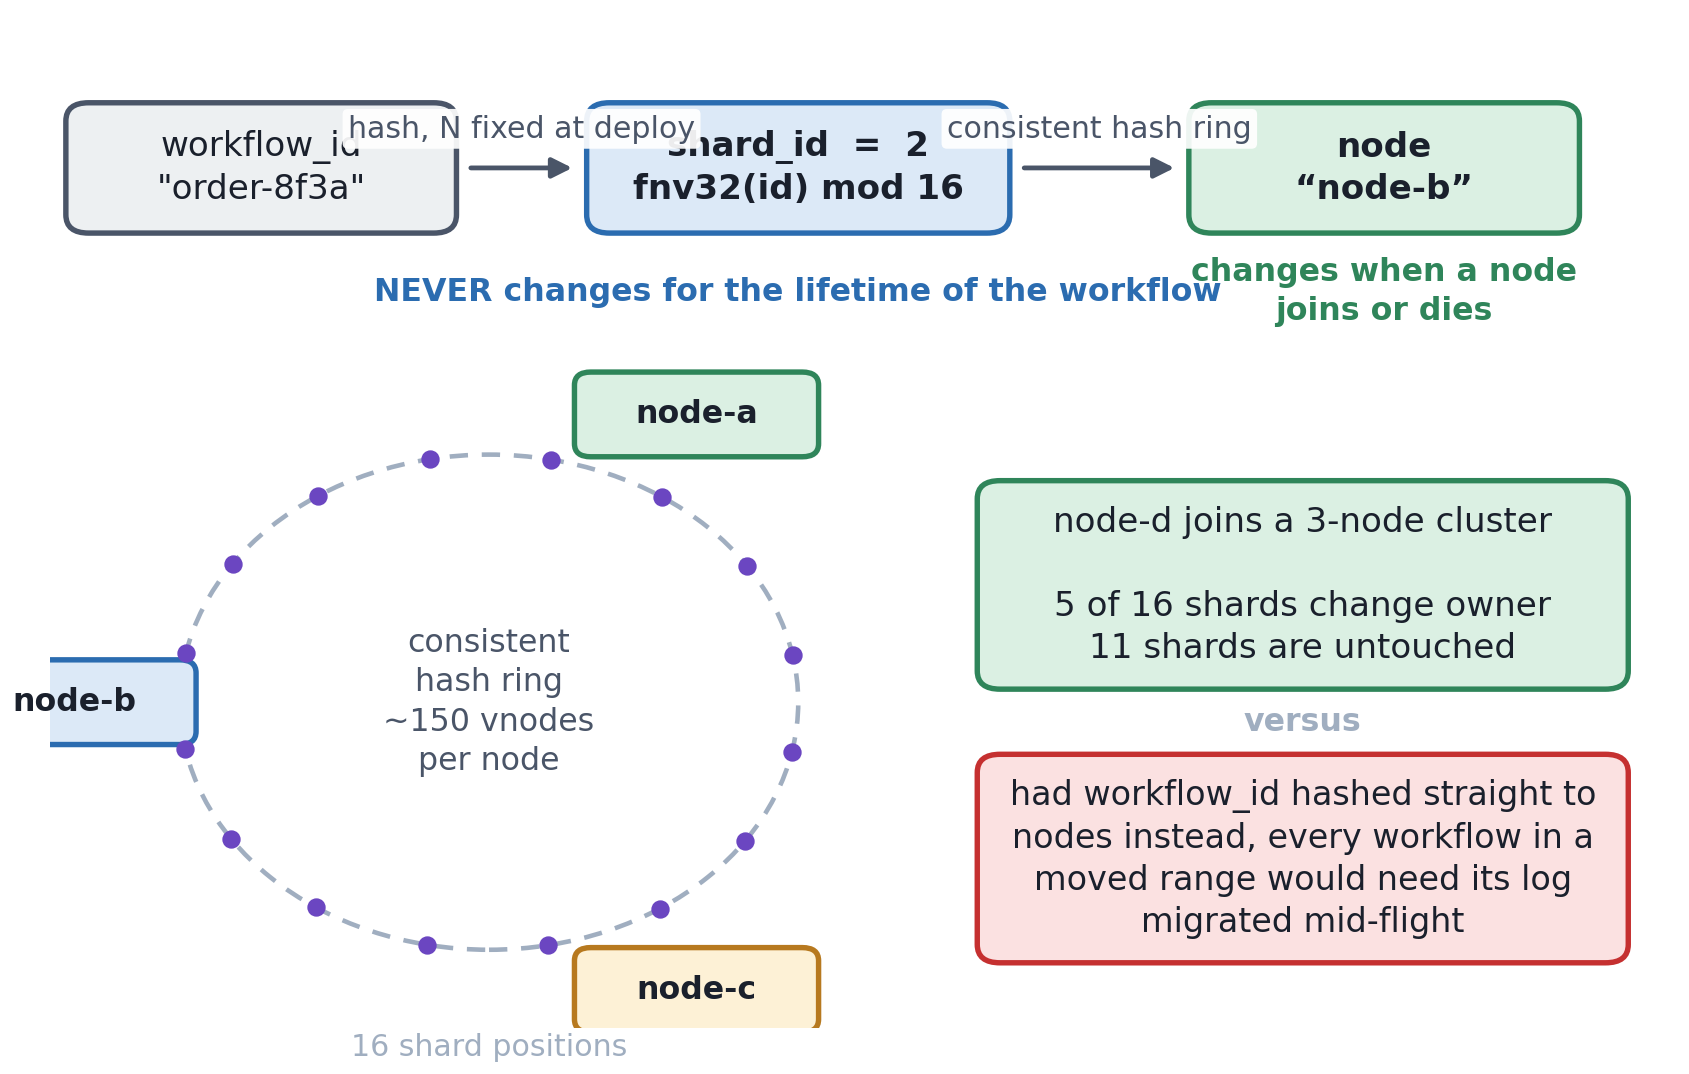
\includegraphics[width=\linewidth]{figures/fig_4_2_two_level_mapping.png}
  \caption{The two-level mapping. The first mapping is fixed for the lifetime
    of a workflow; only the second changes when the cluster is resized. This
    is what reduces rebalancing from a data migration to an ownership
    handoff.}
  \label{fig:mapping}
\end{figure}

\begin{table}[htbp]
  \centering
  \caption{Partitioning parameters and the reasoning behind each default}
  \label{tab:ringparams}
  \small
  \begin{tabular}{@{}p{1.05in}p{0.55in}p{2.82in}@{}}
    \toprule
    \textbf{Parameter} & \textbf{Default} & \textbf{Reasoning} \\
    \midrule
    Shard count $N$ & 16 &
      Must exceed the largest anticipated node count so that every node can
      own at least one shard, but must stay small enough that per-shard
      goroutine overhead is negligible. Fixed at deployment because changing it
      would re-map every workflow. \\
    Virtual nodes per node & $\approx$150 &
      Enough points on the ring for the distribution across physical nodes to
      be near-even; a smaller number produces visible imbalance. \\
    Hash function & FNV-1a, 32-bit &
      Fast, dependency-free and adequate for uniformity. Cryptographic
      strength is not a requirement, because the input is not adversarial. \\
    \bottomrule
  \end{tabular}
\end{table}

\subsection{Ownership, Leases and the Fencing Invariant}

This section contains the central safety argument of the design.

Ownership of a shard is recorded in a single row with four columns: the shard
identifier, the owning node, a monotonically increasing fencing token, and an
expiry timestamp. A node acquires a shard with the conditional update shown in
Listing~\ref{lst:acquire}.

\begin{lstlisting}[language=SQL, caption={Acquiring a shard lease. Zero rows
  returned means another node holds a live lease.}, label={lst:acquire}]
UPDATE shard_leases
SET    owner_node    = $me,
       fencing_token = fencing_token + 1,
       expires_at    = now() + interval '10 seconds'
WHERE  shard_id = $shard
  AND  (owner_node = $me OR expires_at < now())
RETURNING fencing_token;
\end{lstlisting}

Zero rows returned means someone else holds a live lease. One row returned
means the caller owns the shard and now holds token $T$. The token increments
on every change of ownership and never decreases. Renewal, performed every
three seconds against a ten-second expiry, extends \cd{expires\_at} while
requiring both the owner name and the token to match; a renewal returning zero
rows tells the node it has been displaced.

\textbf{The lease is not what makes this safe.} This is the point most often
missed, and it is where naive lease-based designs fail. Consider the following
sequence:

\begin{enumerate}[leftmargin=*, itemsep=1pt]
  \item Node A owns shard 2 with token 7. It polls a task and begins work.
  \item Node A's process freezes --- a garbage-collection pause, a disk stall,
    a virtual-machine suspension. It has no way of knowing that time is
    passing.
  \item Ten seconds elapse. The lease expires. Node B acquires it and receives
    token 8.
  \item Node B replays the workflow and begins executing it.
  \item Node A wakes up mid-transaction, still sincerely believing it holds
    the lease, and attempts to commit.
\end{enumerate}

No amount of care in the lease protocol prevents step five, because node A
cannot detect that it was frozen. What prevents the damage is that every
mutating transaction re-verifies the token \emph{inside the same transaction
as its writes}, as shown in Listing~\ref{lst:fence}.

\begin{lstlisting}[language=Go, caption={The fencing check. Every mutating
  transaction performs this before any write, and \texttt{FOR UPDATE}
  serialises the check against the write.}, label={lst:fence}]
tx, _ := db.Begin()
var tok int64
tx.QueryRow(`SELECT fencing_token FROM shard_leases
             WHERE shard_id = $1 AND owner_node = $2
               AND expires_at > now()
             FOR UPDATE`, shard, me).Scan(&tok)
if tok != myToken {
    tx.Rollback()
    return ErrLostOwnership
}
// ... all event appends, task inserts, timer inserts ...
tx.Commit()
\end{lstlisting}

Node A's transaction reads token 8, compares it against the 7 it believes it
holds, and rolls back. It commits nothing --- not one event, not one task row.
The \cd{FOR UPDATE} clause is what makes this airtight: it serialises the
ownership check against the write, so no window exists between ``check'' and
``write'' during which ownership could change underneath the writer.
Fig.~\ref{fig:fencing} shows the two outcomes side by side.

\begin{figure}[htbp]
  \centering
  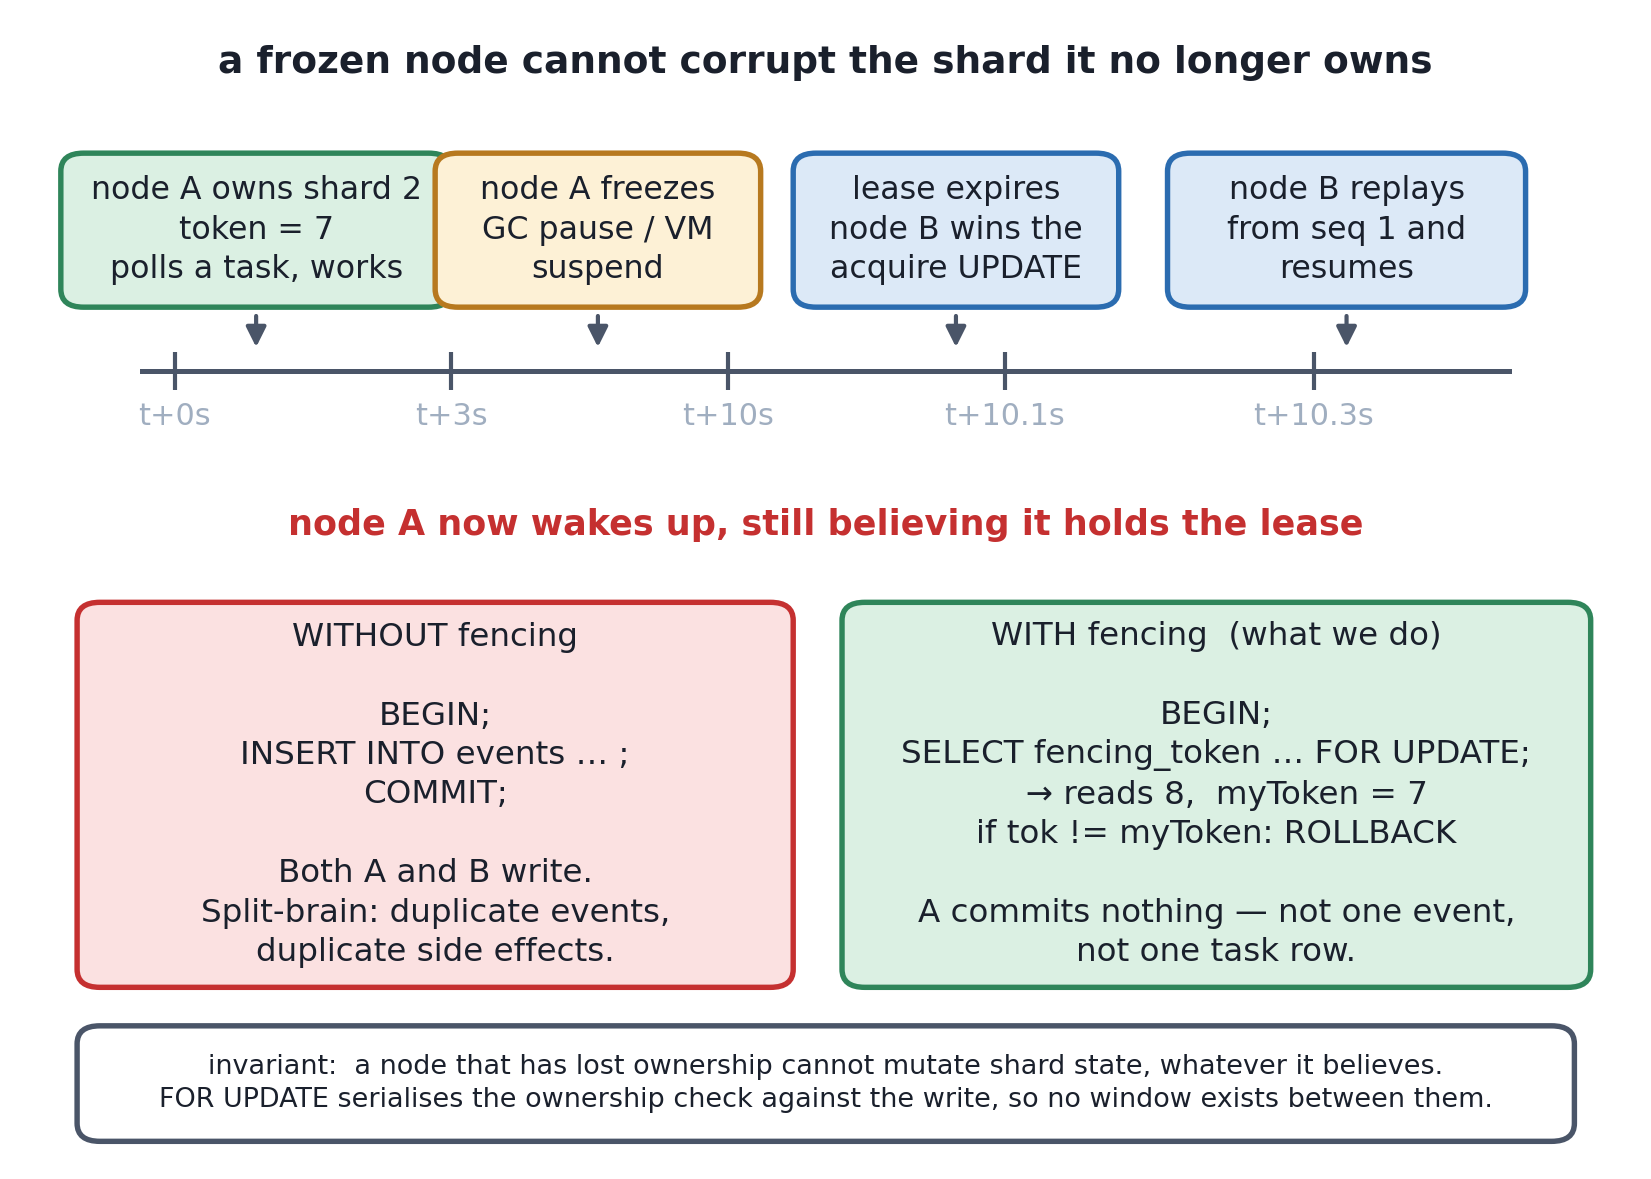
\includegraphics[width=\linewidth]{figures/fig_4_6_lease_fencing.png}
  \caption{Why the lease alone is insufficient and the in-transaction token
    check is what provides safety. Without fencing, a node that was frozen past
    its lease expiry commits alongside the new owner and produces split-brain.
    With fencing, it commits nothing.}
  \label{fig:fencing}
\end{figure}

The resulting invariant, which satisfies FR-8, is:

\begin{quote}
\textbf{A node that has lost ownership cannot mutate shard state, regardless of
what it believes.}
\end{quote}

This is the fencing-token argument~\cite{kleppmann2017} implemented in a table
rather than in ZooKeeper, and it is the same technique Temporal applies under
the name RangeID. Two costs must be stated honestly rather than discovered by
a reader.

\textbf{There is an availability gap.} Between the old owner's death and the
new owner's acquisition, the shard is unavailable for up to one lease
duration. At the default ten-second expiry this bounds unavailability at ten
seconds for $1/N$ of workflows, which is NFR-3. Shortening the lease speeds
failover and increases the risk of spuriously fencing a healthy but momentarily
slow node; this is a genuine tunable trade-off, and the chosen value is a
default rather than a discovery.

\textbf{This is not consensus.} The design relies on PostgreSQL as a single
linearizable source of truth for the ownership record. That is a legitimate
position --- it is the DBOS argument~\cite{dbos2025} --- but it must be stated
plainly: the coordination problem has been moved into the database, not
eliminated, and the database is consequently both the coordination bottleneck
and the availability floor of the whole system.

\subsection{Replication and Failover}

Durability beyond a single machine is obtained from PostgreSQL streaming
replication: a standby receives the write-ahead log from the leader and can be
promoted if the leader is lost.

The choice between asynchronous and synchronous commit is a genuine trade-off
rather than a setting with a right answer. Asynchronous replication
(\cd{synchronous\_commit = off}) is faster but has a loss window: a leader
that dies holding unreplicated commits loses them. Synchronous replication
(\cd{synchronous\_commit = remote\_apply}) has no loss window, but adds a
network round trip to every commit and stalls entirely if the standby is
unavailable. The engine defaults to synchronous commit, treating the
throughput cost as a measurable result rather than as a hidden caveat.

The failover sequence following the loss of a shard-owning node is as follows,
with the default timings:

\begin{enumerate}[leftmargin=*, itemsep=1pt]
  \item $t+0.0$\,s --- the node is killed. In-flight task locks are already
    ticking down.
  \item $t+3.0$\,s --- the dead node misses its first lease renewal.
  \item $t+10.0$\,s --- the lease expires.
  \item $t+10.1$\,s --- a surviving node wins the acquire statement and
    receives the next fencing token.
  \item $t+10.3$\,s --- that node polls a workflow task, replays the history
    from the first event, and resumes.
  \item $t+40.0$\,s --- any activity task locks held by the dead node expire
    and those tasks are redelivered.
\end{enumerate}

Nothing is lost, because nothing was ever held only in the dead node's memory.
Some work may be \emph{repeated}, specifically activities caught in the window
analysed in Section~4.2.8, which is why stable deduplication keys exist.
Recovery time is dominated by the lease expiry and should be reported as a
distribution over many induced failures rather than as a single observation.

Two limitations are recorded here rather than left for a reader to find.
First, \textbf{database failover in this design is slower than published work
and is not automatic}: AMBROSIA~\cite{ambrosia2020} reports automatic failover
in approximately 1.8 seconds with no loss, whereas promotion of the standby in
this system is operator-initiated and takes substantially longer. Second,
shards share one database instance, so the loss of that instance is a
cluster-wide event rather than a per-shard one. Both are consequences of the
single-dependency constraint and both are recorded in Section~1.5.

\subsection{Design Rationale and Rejected Alternatives}

The architecture above is one point in a space of possibilities, and the
decisions that define it are collected here so that they can be assessed
together. The alternatives are tabulated in Table~\ref{tab:stack} of
Chapter~3; this section gives the reasoning for the three decisions that most
shape the design.

\textbf{Why the database and nothing else.} Every mechanism the engine needs
--- an ordered append-only log, a queue with visibility timeouts, a timer
store, and a linearizable compare-and-swap for ownership --- is available
within a single relational database, and crucially they are available
\emph{within one transaction}. Introducing a message broker for the queue or a
coordination service for ownership would mean that a workflow decision and its
consequences could no longer be committed atomically, and the engine would
have to implement the missing atomicity itself. The dependency count would
rise and the complexity would rise with it. This reasoning is what makes
NFR-6 a design asset rather than an arbitrary restriction.

\textbf{Why ownership is a lease rather than consensus.} A full consensus
protocol would remove the dependence on a single database as the arbiter of
ownership. It would also require operating a second distributed system, which
contradicts the project's central thesis. Because the fencing check makes a
displaced node harmless regardless of what it believes, the weaker mechanism
is sufficient for the safety property the system actually needs. Consensus
would improve availability, not correctness, and availability is explicitly
bounded rather than maximised in NFR-3.

\textbf{Why compensation rather than locking.} Holding database locks for the
duration of a multi-step workflow would provide isolation between concurrent
workflows, which sagas do not. AC/DC~\cite{acdc2026} measured the cost of that
approach directly: with one-second steps their locking variant degraded to
approximately two orders per second with 42\% of orders failing, while
compensation sustained sixteen orders per second with no failures. The
isolation gap that sagas leave is real, and is acknowledged in Section~4.2.9
rather than solved.

% =====================================================================
%  CHAPTER 4, SECTION 4.2 — LOW LEVEL DESIGN
%  Included from parts/ch4.tex
% =====================================================================

\section{Low Level Design}

This section descends from the architecture to the mechanisms. It specifies
the tables that hold every piece of durable state, the loop that executes a
workflow, the device by which replay is matched to history, the concurrency
handshake inside a worker, the failure analysis that bounds what the engine
can promise, and the decision path of the semantic idempotency contribution.

\subsection{Persistent Data Model}

All durable state in the system lives in six tables, shown in
Fig.~\ref{fig:schema}. There is one PostgreSQL database for the whole cluster
rather than one per shard: sharding is physically expressed as the
\cd{shard\_id} column that every table carries, and what confines a node to
its own shards is the lease it holds together with the \cd{shard\_id} present
in every statement it issues.

\begin{figure}[htbp]
  \centering
  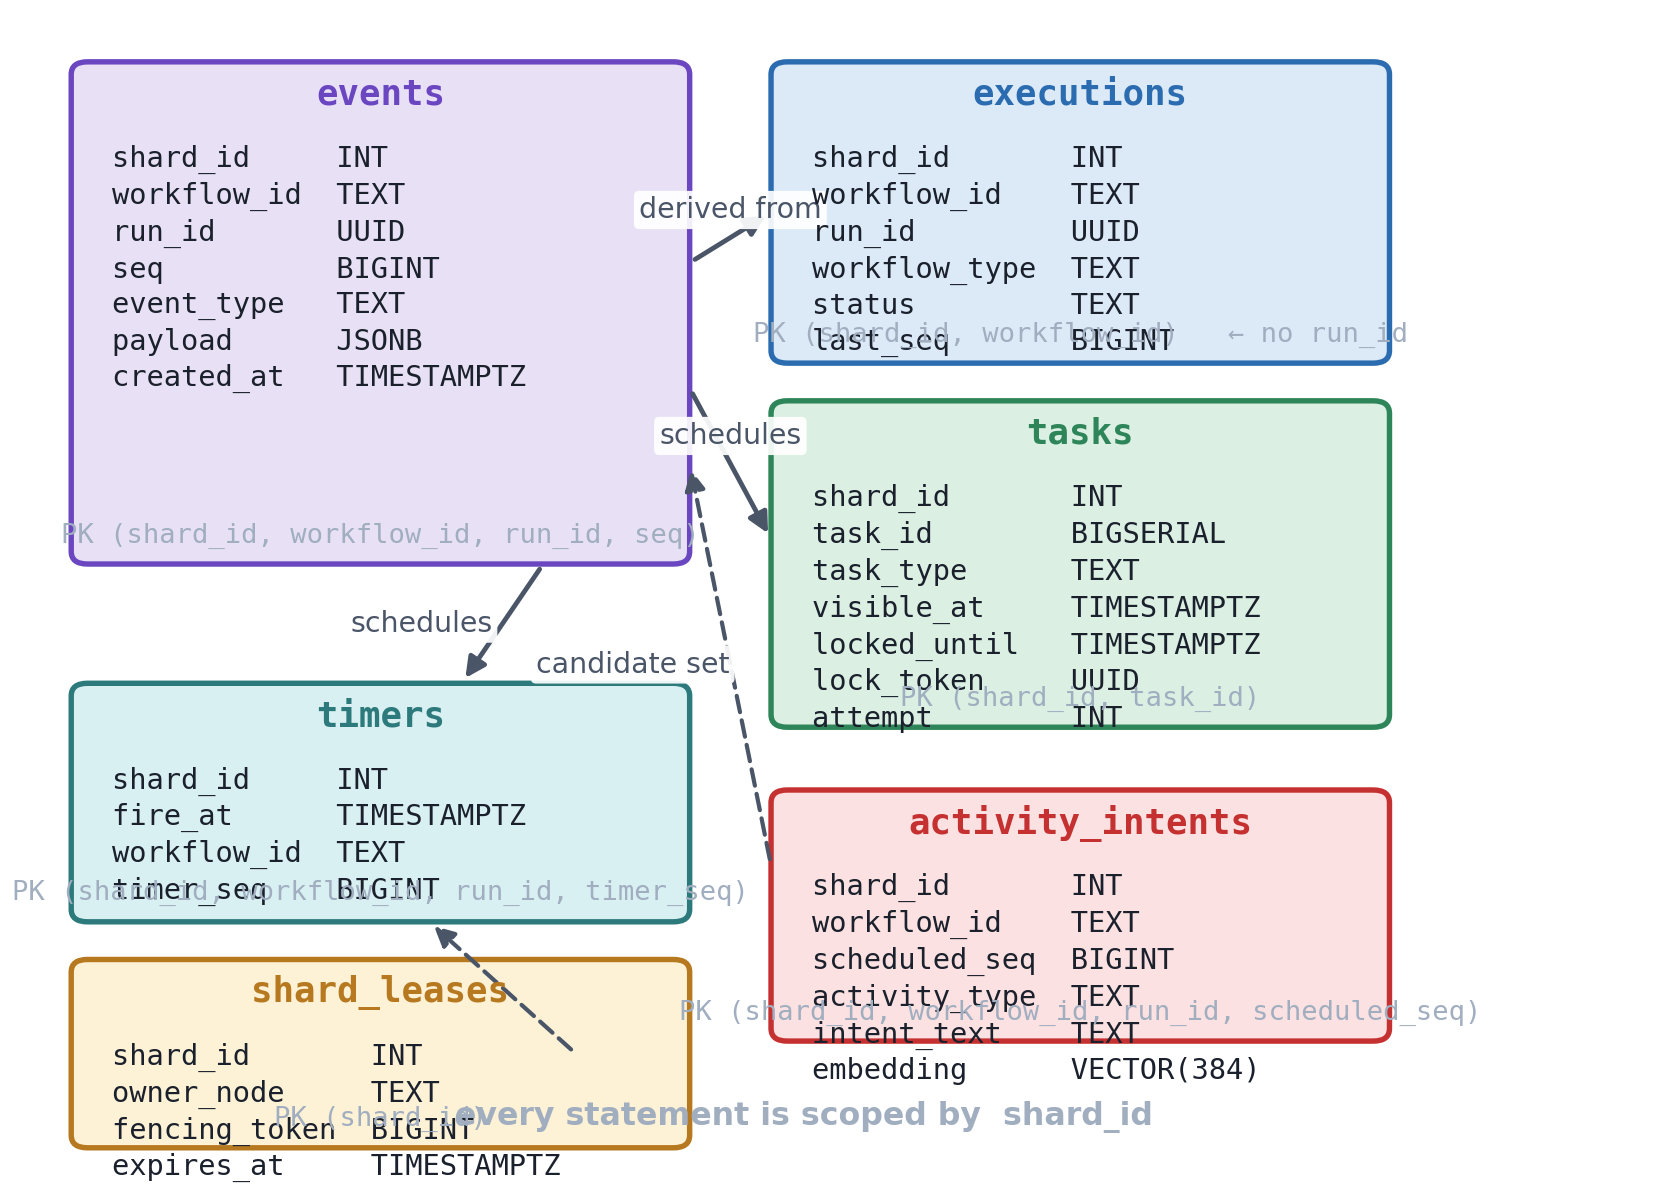
\includegraphics[width=\linewidth]{figures/fig_4_4_schema.png}
  \caption{The six tables holding every piece of durable state in the system.
    Every table carries \texttt{shard\_id}, which is what sharding physically
    is in this design; no statement is ever issued without it.}
  \label{fig:schema}
\end{figure}

\subsubsection{The event log}

\begin{lstlisting}[language=SQL, caption={The event log. The primary key
  provides append-only semantics without any explicit
  locking.}, label={lst:events}]
CREATE TABLE events (
    shard_id    INT         NOT NULL,
    workflow_id TEXT        NOT NULL,
    run_id      UUID        NOT NULL,
    seq         BIGINT      NOT NULL,  -- 1, 2, 3, ... per (workflow_id, run_id)
    event_type  TEXT        NOT NULL,
    payload     JSONB       NOT NULL,
    created_at  TIMESTAMPTZ NOT NULL DEFAULT now(),
    PRIMARY KEY (shard_id, workflow_id, run_id, seq)
);
\end{lstlisting}

Three properties of Listing~\ref{lst:events} are load-bearing rather than
incidental.

\textbf{The primary key provides append-only semantics for free.} If two
workers both attempt to append sequence number 47 for the same run, exactly
one succeeds and the other receives a unique-constraint violation and rolls
back. No lock is required to protect the log, because the primary key
\emph{is} the concurrency control. This is the cheapest correctness guarantee
available in the whole design, and it is obtained at no cost.

\textbf{The \cd{run\_id} column exists so that a workflow identifier can be
re-run.} A business key such as \cd{order-8f3a} may be retried as a fresh
execution after a terminal failure. The workflow identifier is the stable,
user-facing business key; the run identifier denotes one attempt at it.

\textbf{No \cd{UPDATE} is ever issued against this table.} The absence is
checked by an automated assertion (FR-1), because an update to the log would
mean that history could be rewritten, and every guarantee in this chapter
would become conditional.

\subsubsection{The execution pointer}

The log is the truth, but scanning the whole log to answer ``is this order
still running?'' would be prohibitive. The \cd{executions} table therefore
holds one mutable row per workflow, derived from the log, carrying the
workflow type, its status and the highest sequence number written.

Its primary key is \cd{(shard\_id, workflow\_id)} and deliberately excludes
\cd{run\_id}. The effect is that at most one open run may exist per business
key, which makes starting a workflow idempotent at the front door: a duplicate
start request collides with the unique constraint and the engine returns the
existing execution rather than creating a second one. This is free
deduplication obtained from the schema rather than from application logic.

\subsubsection{Event types}

\begin{table}[p]
  \centering
  \caption{Event types written to the log, grouped by the mechanism that
    produces them}
  \label{tab:eventtypes}
  \small
  \begin{tabular}{@{}p{1.95in}p{0.68in}p{2.0in}@{}}
    \toprule
    \textbf{Event type} & \textbf{Group} & \textbf{Meaning} \\
    \midrule
    \cd{WorkflowExecutionStarted} & Lifecycle & A run has begun; carries the
      workflow type and input \\
    \cd{WorkflowExecutionCompleted} & Lifecycle & Terminal success \\
    \cd{WorkflowExecutionFailed} & Lifecycle & Terminal failure \\
    \cd{ActivityTaskScheduled} & Activity & The intent to perform a side
      effect, recorded \emph{before} it occurs; carries $k$ and the dedup key \\
    \cd{ActivityTaskCompleted} & Activity & The side effect succeeded; carries
      its result \\
    \cd{ActivityTaskFailed} & Activity & The attempt failed; drives the retry
      policy \\
    \cd{TimerStarted} & Timer & A durable sleep has begun \\
    \cd{TimerFired} & Timer & The sleep has elapsed \\
    \cd{SignalReceived} & Signal & An external event was delivered into the
      workflow \\
    \cd{SideEffectRecorded} & Determinism & A non-deterministic value, computed
      once and journalled \\
    \cd{SemanticDedupEvaluated} & Idempotency & A deduplication verdict with
      its similarity, threshold and matched predecessor \\
    \cd{CompensationScheduled} & Saga & A compensating action has been
      scheduled \\
    \cd{CompensationCompleted} & Saga & A compensating action succeeded \\
    \cd{CompensationFailed} & Saga & A compensating action exhausted its
      retries \\
    \cd{CompensationResumed} & Saga & Compensation continued after a recovery \\
    \bottomrule
  \end{tabular}
\end{table}

\subsection{The Workflow Task Loop}

A \emph{workflow task} means precisely one thing: \emph{this workflow has new
history; run its code forward until it blocks again}. The loop that processes
one such task, shown in Fig.~\ref{fig:taskloop}, is the heart of the engine.

\begin{figure}[htbp]
  \centering
  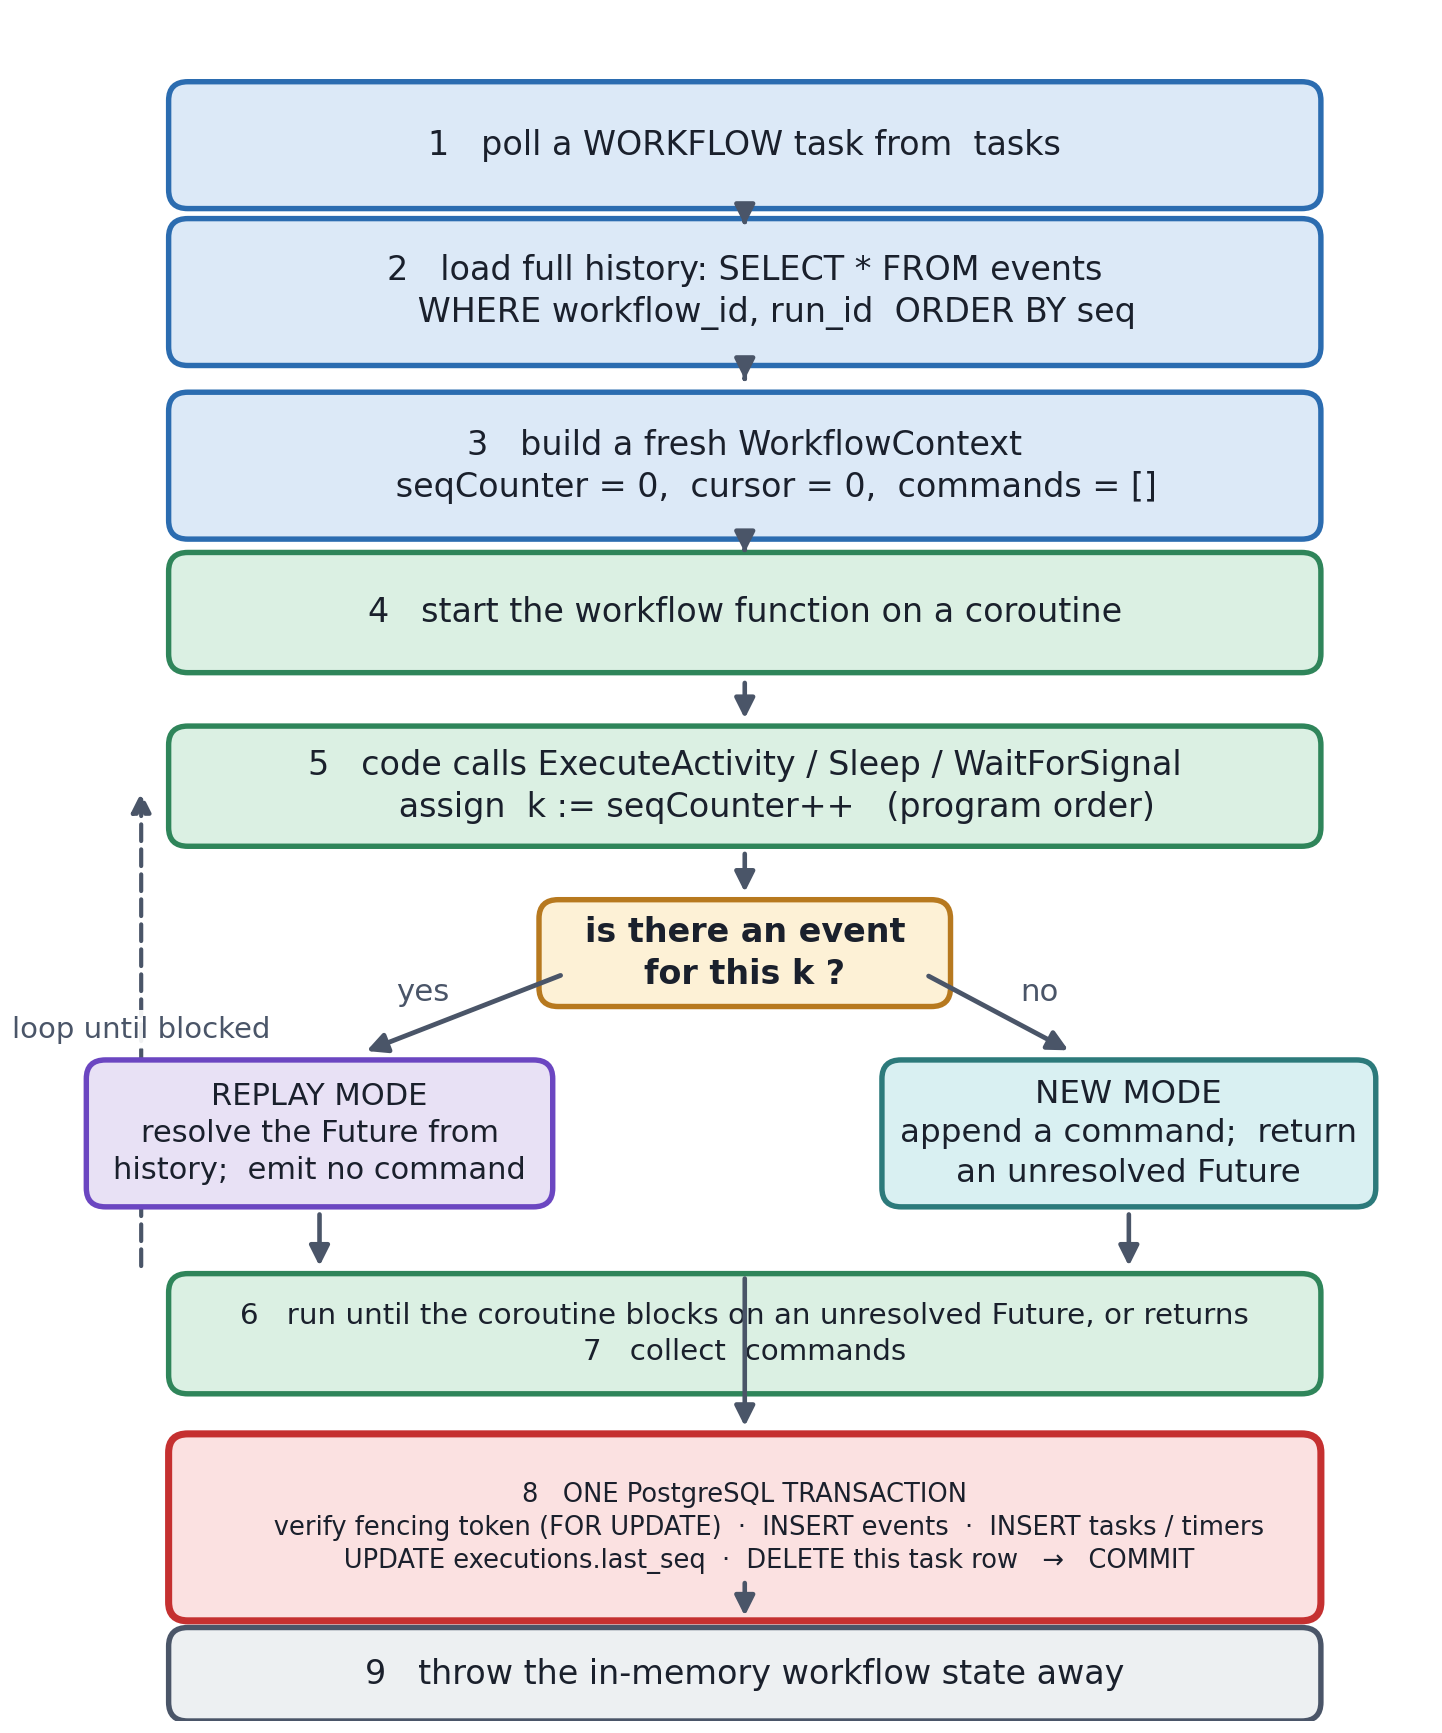
\includegraphics[height=0.80\textheight,keepaspectratio]{figures/fig_4_3_task_loop.png}
  \caption{The workflow task loop. Step 8 is a single transaction, which is
    what makes the system safe; step 9 discards the in-memory state, which is
    why correctness never depends on retaining it.}
  \label{fig:taskloop}
\end{figure}

Two steps deserve particular attention.

\textbf{Step 8 is one transaction.} The fencing-token verification, the
insertion of every event implied by the decisions just made, the insertion of
the corresponding task and timer rows, the update of the execution pointer,
and the deletion of the workflow task row all commit together or not at all.
Either the decision and every one of its consequences lands, or none of it
does. There is no partial state to reconcile, ever, and no reconciliation code
exists anywhere in the engine because none can be needed.

\textbf{Step 9 is not an oversight.} The in-memory workflow state is thrown
away after every task. Correctness never depends on keeping it. This is what
permits any node to pick up any workflow task at any moment without
coordination, and it is what makes shard failover a matter of ownership rather
than of state transfer.

\subsection{Program Order as the Replay Join Key}

Replay requires a way of matching ``the call the code is making right now'' to
``the event that recorded that call last time''. The mechanism is a counter,
and it is the device most often missed in descriptions of durable execution.

\begin{lstlisting}[language=Go, caption={Program order. The counter $k$ is
  incremented once per call, in the order the code makes the calls, and
  appears nowhere in the source.}, label={lst:progorder}]
func (w *FoodDeliveryWorkflow) Execute(ctx WorkflowContext) error {
    if err := ctx.ExecuteActivity("ChargePayment", w.order).Get(); err != nil {
        return err                                                    // k = 0
    }
    if err := ctx.ExecuteActivity("NotifyRestaurant", w.order).Get(); err != nil {
        return ctx.ExecuteActivity("RefundPayment", w.order).Get()    // k = 1, 2
    }
    return nil
}
\end{lstlisting}

The value $k$ is assigned by a counter incremented once per call, in the order
the code makes the calls. It is recomputed identically on every replay because
the code takes the same branches; the code takes the same branches because it
is deterministic; and it is deterministic because it reads only from history.
The value is written into the \cd{ActivityTaskScheduled} payload, and on
replay it is the join key between the live call and the recorded event.

If the code takes a different branch on replay --- because it was edited, or
because it consulted something non-deterministic --- then $k$ shifts, the match
fails, and the engine raises a \emph{non-determinism error}. The engine cannot
repair this condition and does not attempt to. It has no way of knowing which
version of the code told the truth, and any attempted reconciliation would
corrupt the history silently. It therefore refuses to continue, which is the
behaviour required by FR-3.

\subsection{The Cooperative Scheduler}

A call to \cd{future.Get()} must suspend the workflow \emph{without} blocking
an operating-system thread and \emph{without} handing scheduling control to
the Go runtime in a way the engine cannot predict. What is required is
cooperative, deterministic scheduling, obtained through the two-channel
handshake in Listing~\ref{lst:coroutine}.

\begin{lstlisting}[language=Go, caption={The dispatcher--workflow handshake.
  Exactly one goroutine is runnable at any instant.}, label={lst:coroutine}]
type coroutine struct {
    unblock chan struct{}   // dispatcher -> workflow: "keep going"
    yielded chan struct{}   // workflow -> dispatcher: "I am blocked"
}

// Called from workflow code, on the workflow goroutine.
func (f *future) Get() (any, error) {
    for !f.ready {
        f.co.yielded <- struct{}{}   // hand control to the dispatcher
        <-f.co.unblock               // wait to be resumed
    }
    return f.value, f.err
}

// Dispatcher, on the engine goroutine.
func (d *dispatcher) runUntilBlocked() {
    d.co.unblock <- struct{}{}   // let the workflow run
    <-d.co.yielded               // it ran until it blocked or finished
}
\end{lstlisting}

The two goroutines ping-pong, and exactly one is runnable at any instant.
There is no true parallelism inside a workflow, and that is precisely the
point: parallelism would be non-determinism. This also explains why
\cd{go func()\{\}}, \cd{time.Sleep}, \cd{sync.Mutex} and raw channels are
forbidden inside workflow code --- each hands scheduling to the Go runtime,
which does not consult the event history.

\subsection{Determinism in Practice}

Determinism is a property of the workflow code, which the engine can detect
violations of but cannot enforce in advance. Table~\ref{tab:determinism} lists
the constructs that break it and the replacement provided for each.

\begin{table}[htbp]
  \centering
  \caption{Constructs forbidden in workflow code, and their replacements}
  \label{tab:determinism}
  \small
  \begin{tabular}{@{}p{1.0in}p{1.7in}p{1.85in}@{}}
    \toprule
    \textbf{Forbidden} & \textbf{Why} & \textbf{Replacement} \\
    \midrule
    \cd{time.Now()} & Differs on every replay &
      \cd{ctx.Now()}, returning the timestamp recorded in the event log \\
    \cd{rand}, \cd{uuid.New()} & Differs on every replay &
      \cd{ctx.SideEffect(fn)}, which journals the result \\
    \cd{time.Sleep} & Blocks a real thread and depends on wall-clock time &
      \cd{ctx.Sleep(d)}, a durable timer \\
    \cd{go func()\{\}} & Non-deterministic interleaving &
      \cd{ctx.Go()} on the same cooperative scheduler \\
    Map iteration & Go randomises map ordering deliberately &
      Sort the keys before iterating \\
    Environment, files, network & The environment differs across machines &
      Perform it inside an activity \\
    Global mutable state & Shared across replays &
      Pass it through the workflow input \\
    \bottomrule
  \end{tabular}
\end{table}

The escape hatch, \cd{SideEffect}, is the general solution to unavoidable
non-determinism, and is worth stating precisely because Section~4.2.10 is an
application of it. In new mode the engine runs the supplied closure, obtains
its value, appends a \cd{SideEffectRecorded} event carrying $k$ and that
value, and returns it. In replay mode the engine does \emph{not} run the
closure; it reads the value out of the recorded event and returns that.
Non-determinism is thereby neutralised by journalling its result.

The map-iteration entry deserves a specific warning. Go randomises map
iteration order deliberately, so a loop that schedules activities while
ranging over a map will schedule them in a different order on replay and
produce a non-determinism error --- intermittently, perhaps once in twenty
runs. Sorting the keys is the fix.

\subsection{A Worked Execution Trace}

The mechanisms above are best understood through a concrete trace.
Fig.~\ref{fig:sequence} follows one workflow, \cd{order-8f3a}, which hashes to
shard~2, across its first three tasks.

\begin{figure}[htbp]
  \centering
  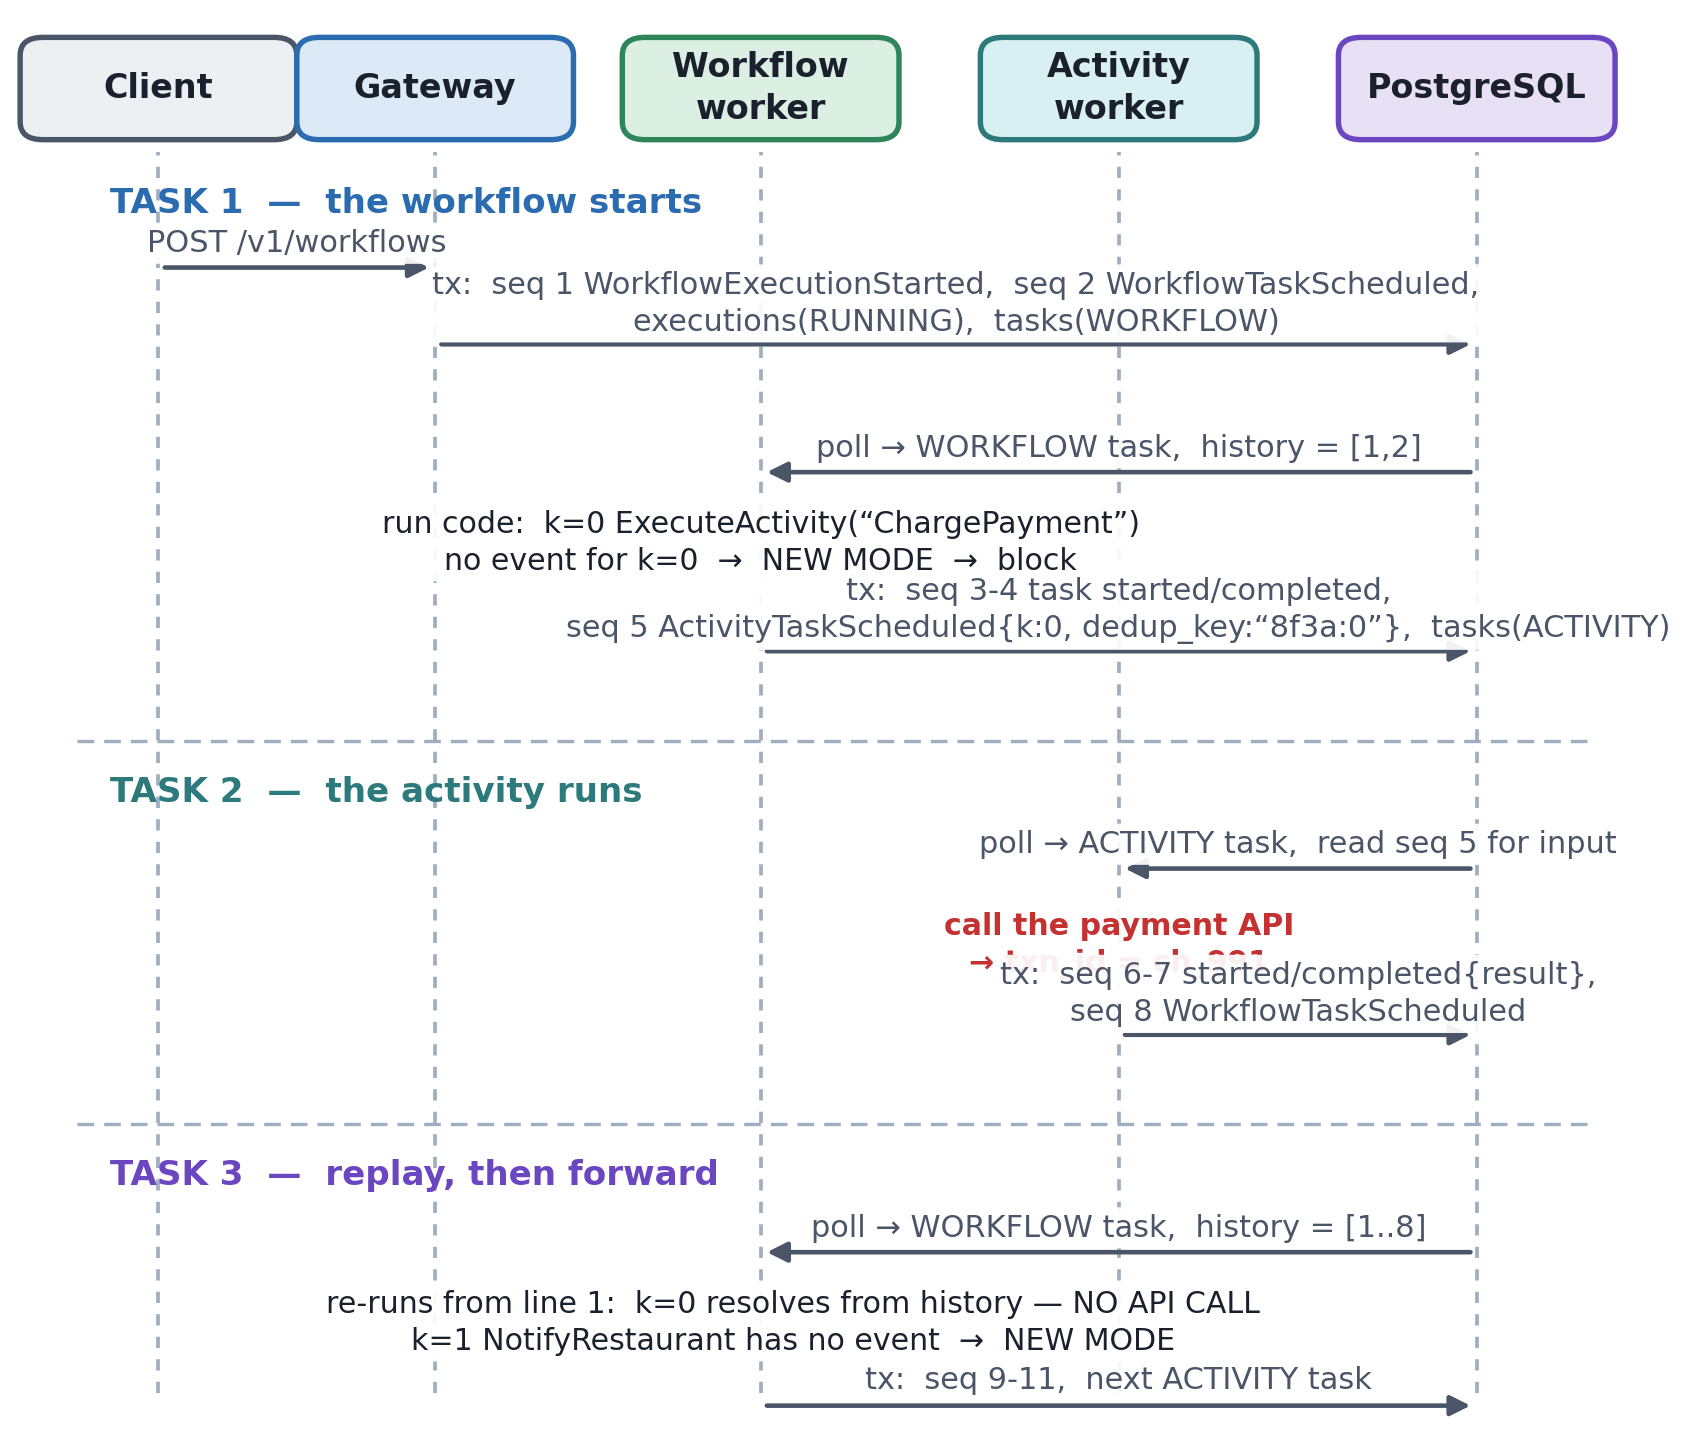
\includegraphics[width=\linewidth]{figures/fig_4_5_sequence.png}
  \caption{A worked trace across three tasks. The crucial moment is the
    writing of sequence 5: the \emph{intent} to charge is durably recorded
    before any money moves, which is the entire basis of the engine's safety.}
  \label{fig:sequence}
\end{figure}

\textbf{Task 1 --- the workflow starts.} The gateway writes, in one
transaction, two events --- a workflow-started event at sequence 1 and a
workflow-task-scheduled event at sequence 2 --- together with a task row and
an execution row. A workflow worker polls that task and sees a history of two
events. It runs the code: the first call,
\cd{ExecuteActivity("ChargePayment")}, is assigned $k=0$; no event for $k=0$
exists in history, so the engine is in new mode; it emits a command and returns
an unresolved future. The code calls \cd{Get()} and blocks. The dispatcher
regains control, finds no more history to feed, and the task is complete. The
commit appends sequences 3 through 5 and inserts an activity task row.

Sequence 5 is the critical row of the whole trace, and
Table~\ref{tab:trace1} shows it. \textbf{The intent to charge has been durably
recorded before anything was charged.} That ordering is the basis of every
safety property the engine claims.

\begin{table}[htbp]
  \centering
  \caption{The events written when the first workflow task commits}
  \label{tab:trace1}
  \small
  \begin{tabular}{@{}p{0.3in}p{1.45in}p{2.72in}@{}}
    \toprule
    \textbf{seq} & \textbf{event\_type} & \textbf{payload} \\
    \midrule
    3 & \cd{WorkflowTaskStarted} & \cd{\{"worker":"node-a"\}} \\
    4 & \cd{WorkflowTaskCompleted} & \cd{\{\}} \\
    5 & \cd{ActivityTaskScheduled} &
      \cd{\{"k":0, "activity":"ChargePayment",}
      \cd{"input":\{\ldots\}, "dedup\_key":"8f3a:0"\}} \\
    \bottomrule
  \end{tabular}
\end{table}

\textbf{Task 2 --- the activity runs.} An activity worker polls the activity
task, reads sequence 5 for its input, and calls the payment API, which
succeeds. The worker appends \cd{ActivityTaskStarted}, then
\cd{ActivityTaskCompleted} carrying the result, then a fresh
\cd{WorkflowTaskScheduled}; it deletes the activity task row and inserts a
workflow task row. The result is now in history and will never be recomputed.

\textbf{Task 3 --- replay, then forward.} A worker polls the workflow task and
sees a history of eight events. \emph{It runs the workflow function from the
very first line again.} The call at $k=0$ finds both
\cd{ActivityTaskScheduled} and \cd{ActivityTaskCompleted} in history, so the
engine is in replay mode: the future resolves immediately with the recorded
result and \textbf{no API call is made}. The code never knows the difference.
Execution continues past the point previously reached, the call at $k=1$ finds
nothing in history, and the engine returns to new mode.

That is the complete engine. Everything remaining in this section makes it
survive progressively worse failures.

\subsection{The Durable Task Queue}

Work is dispatched through a table rather than a message broker. The table
carries a visibility timestamp, a lock expiry, a lock token and an attempt
counter. Critically it is a \emph{lease queue} rather than a delete-on-read
queue: a worker does not remove the row, it takes a time-boxed lock on it. If
the worker dies, the lock expires and the task becomes visible again. That is
the entire crash-recovery story for in-flight tasks, and it requires no
detection mechanism and no timeout thread.

\begin{lstlisting}[language=SQL, caption={The poll query. \texttt{SKIP LOCKED}
  is what allows many workers to dequeue concurrently without serialising
  behind a single row lock.}, label={lst:poll}]
UPDATE tasks
SET    locked_until = now() + interval '30 seconds',
       lock_token   = gen_random_uuid(),
       attempt      = attempt + 1
WHERE  (shard_id, task_id) IN (
    SELECT shard_id, task_id FROM tasks
    WHERE  shard_id = $1
      AND  task_type = $2
      AND  visible_at <= now()
      AND  (locked_until IS NULL OR locked_until < now())
    ORDER BY task_id
    FOR UPDATE SKIP LOCKED
    LIMIT 1
)
RETURNING *;
\end{lstlisting}

The \cd{SKIP LOCKED} clause in Listing~\ref{lst:poll} is not an optimisation.
Without it, every worker attempting to poll would queue behind the same row
lock and the system would serialise regardless of how many workers were
running; with it, each worker skips rows already locked by another and the
queue scales with worker count. This single clause is the reason the design
can satisfy NFR-6 without an external broker.

Delayed retries require no additional mechanism: a retry is an ordinary row
whose \cd{visible\_at} is set to a future time. The queue already understands
delay.

\subsection{Durable Timers and Signals}

\subsubsection{Timers}

A call to \cd{ctx.Sleep(5 * time.Minute)} at $k=3$ proceeds as follows. In new
mode the engine appends \cd{TimerStarted} carrying $k$ and the firing time,
inserts a row into the timer table, and returns an unresolved future; the
workflow blocks and the worker moves on to other work. \textbf{Nothing holds a
thread, a connection or a byte of memory for those five minutes.} A background
scanner per shard polls for timers whose firing time has passed, and for each
one appends \cd{TimerFired}, deletes the timer row and inserts a workflow task
--- all in one transaction. The workflow task then replays from the first
event, finds both \cd{TimerStarted} and \cd{TimerFired} at $k=3$, resolves the
future immediately and continues.

A five-minute sleep and a five-day sleep therefore cost exactly the same, and
a cluster restart during the wait is invisible, because the timer is a row
rather than a thread.

\subsubsection{Racing a timer against an activity}

A common requirement --- ``wait up to five minutes for the restaurant to
respond'' --- is expressed as a selector over two futures. The selector must
resolve \textbf{in history order}, not in whichever-fires-first order.
Resolving by arrival would mean the branch taken during the live run could
differ from the branch taken during replay, which is precisely a
non-determinism error. The engine therefore resolves a selector by scanning
history for whichever completion event carries the lower sequence number.

\subsubsection{Signals}

A signal is an external event injected into a running workflow: a restaurant
accepting an order, or a human approving an agent's plan. On receipt the
engine routes to the owning shard, verifies the fencing token, appends
\cd{SignalReceived}, inserts a workflow task, and commits. The signal is
durable \emph{before} any workflow code observes it, so if the entire cluster
dies one millisecond later the signal is not lost (FR-11).

Signals that arrive before the workflow has reached the corresponding wait
must still be delivered. They are buffered in history and matched by name
rather than by arrival order relative to $k$. Failing to do this is the
classic defect in hand-rolled implementations of this mechanism.

\subsection{Retry Semantics and the Crash-Window Analysis}

This subsection contains the engine's most important honest claim, and it is
stated before the evidence rather than after it:

\begin{quote}
\textbf{The engine provides at-least-once execution of activities and
exactly-once observation of their results.} True exactly-once execution across
a process boundary is impossible; the engine's role is to make the boundary
narrow and to hand the application the tool with which to close it.
\end{quote}

The proof is a catalogue of every place a crash can land during the execution
of one activity. Fig.~\ref{fig:crashwin} shows the four windows on a timeline
and Table~\ref{tab:crashwindows} gives them in full.

\begin{figure}[htbp]
  \centering
  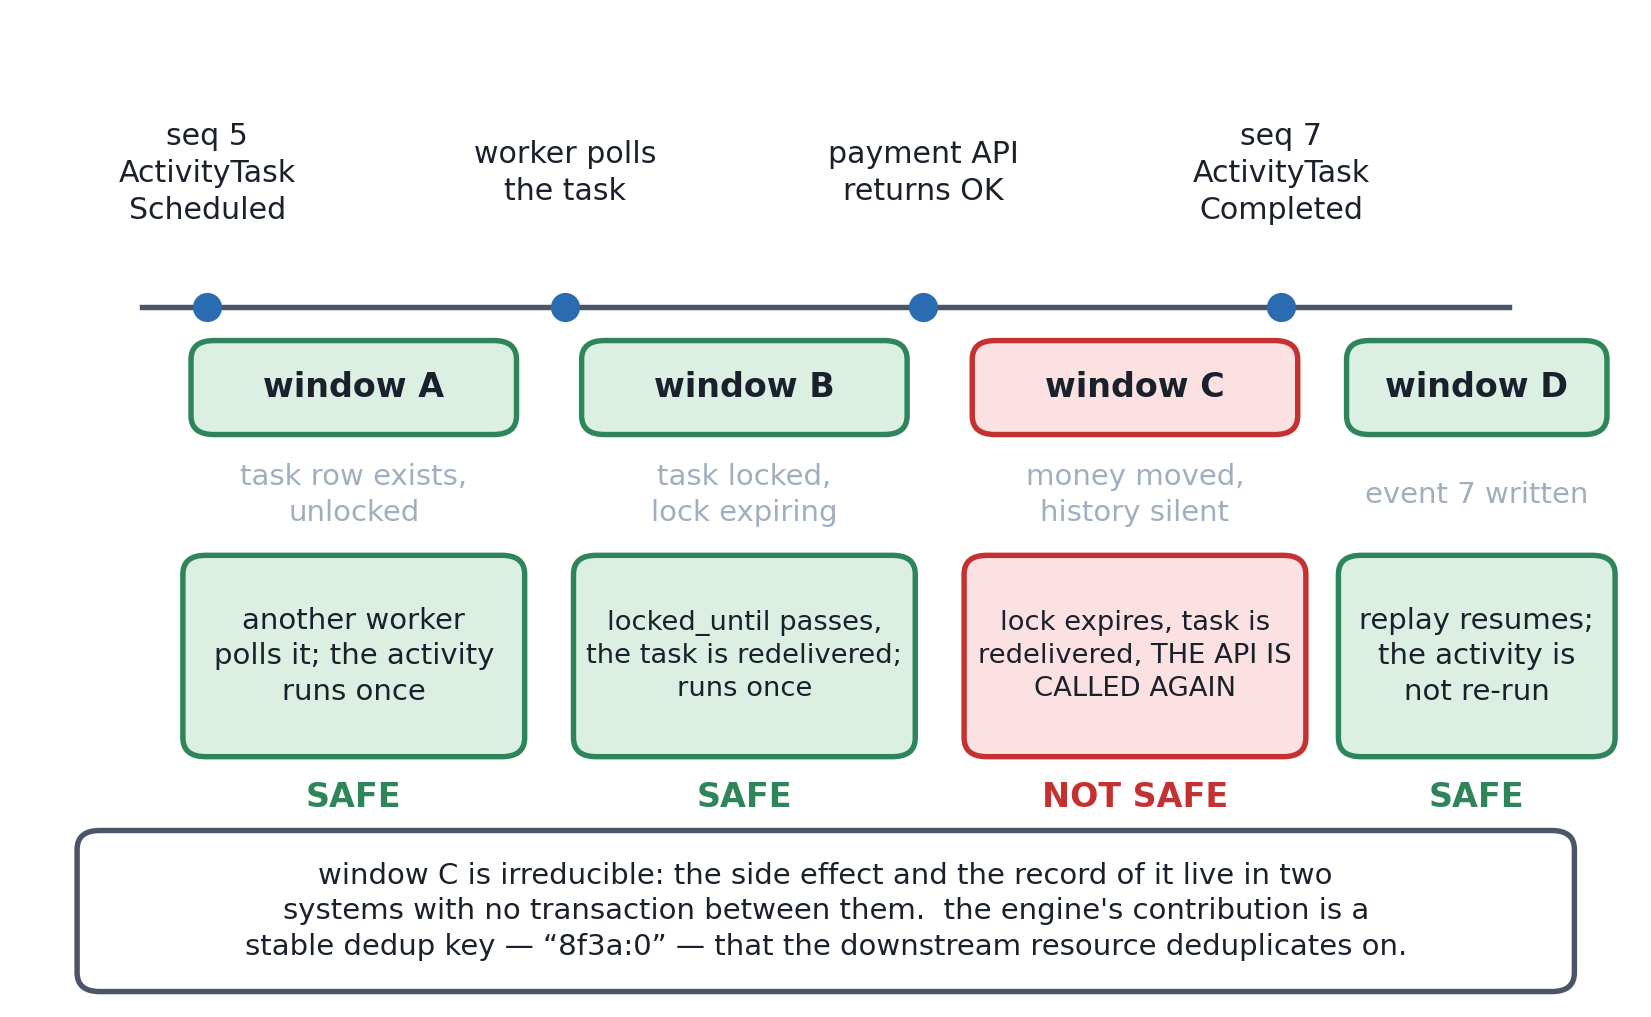
\includegraphics[width=\linewidth]{figures/fig_4_7_crash_windows.png}
  \caption{Every place a crash can land during one activity. Three of the four
    windows recover safely without intervention. Window C is irreducible, and
    the design says so rather than claiming exactly-once execution.}
  \label{fig:crashwin}
\end{figure}

\begin{table}[htbp]
  \centering
  \caption{Crash-window analysis for a single activity execution}
  \label{tab:crashwindows}
  \small
  \begin{tabular}{@{}p{0.18in}p{1.22in}p{1.05in}p{1.5in}p{0.5in}@{}}
    \toprule
    & \textbf{Crash point} & \textbf{State on disk} & \textbf{On recovery} &
    \textbf{Safe?} \\
    \midrule
    A & After the activity is scheduled, before any worker polls &
      Task row exists, unlocked &
      Another worker polls it; the activity runs once & Yes \\
    B & Worker polled the task, crashed before calling the API &
      Task locked, lock expiring &
      The lock expires, the task is redelivered, the activity runs once & Yes \\
    C & \textbf{The API succeeded; the worker crashed before writing the
      completion event} &
      Task locked; money has moved; history is silent &
      The lock expires, the task is redelivered, \textbf{and the worker calls
      the API a second time} & \textbf{No} \\
    D & The completion event was written; crash before the workflow task is
      processed & Workflow task row exists &
      Redelivered; replay resumes; the activity is not re-run & Yes \\
    \bottomrule
  \end{tabular}
\end{table}

Window C is irreducible. The side effect and the record of it live in two
different systems, and there is no distributed transaction spanning the
engine's database and a third-party payment processor. The same conclusion is
reached independently by DBOS~\cite{dbos2025} and R3~\cite{r3vldb2023}. What
the engine does about it is threefold:

\begin{enumerate}[leftmargin=*, itemsep=1pt]
  \item It derives a stable \textbf{deduplication key} --- \cd{"8f3a:0"} ---
    from the workflow identifier and the deterministic $k$. The key is
    identical on every retry, because $k$ is stable across replays.
  \item It passes that key to the activity, which forwards it as the
    downstream service's idempotency key.
  \item The downstream service performs the actual deduplication.
\end{enumerate}

The engine's contribution is therefore precisely \emph{generating a key that
is stable across crashes, retries and replays}, which the application could
not have generated on its own, because the application does not know its own
program order. The final deduplication happens where it must, at the resource.
Being explicit about this division is a strength of the design rather than a
concession.

\begin{table}[htbp]
  \centering
  \caption{Retry policy parameters, evaluated by the workflow worker on seeing
    an activity failure}
  \label{tab:retry}
  \small
  \begin{tabular}{@{}p{1.35in}p{0.6in}p{2.48in}@{}}
    \toprule
    \textbf{Parameter} & \textbf{Default} & \textbf{Effect} \\
    \midrule
    \cd{InitialInterval} & 1\,s & Delay before the first retry \\
    \cd{BackoffCoefficient} & 2.0 & Multiplier applied to each successive delay \\
    \cd{MaximumInterval} & 100\,s & Ceiling on the computed delay \\
    \cd{MaximumAttempts} & 5 & Zero means unlimited \\
    \cd{NonRetryableErrors} & empty &
      Error types that terminate immediately, such as an invalid card, for
      which retrying cannot succeed \\
    \bottomrule
  \end{tabular}
\end{table}

\subsection{Saga Compensation}

Compensation is not a separate engine subsystem. It is a workflow pattern that
the engine makes durable, and understanding that is the point of this
subsection.

\begin{lstlisting}[language=Go, caption={Saga compensation. Each compensation
  is registered only \emph{after} the forward step it undoes has
  succeeded.}, label={lst:saga}]
func (w *FoodDeliveryWorkflow) Execute(ctx WorkflowContext) error {
    saga := NewSaga(ctx)
    defer saga.Cleanup()

    if err := ctx.ExecuteActivity("ChargePayment", w.order).Get(); err != nil {
        return err                                 // nothing done, nothing to undo
    }
    saga.AddCompensation("RefundPayment", w.order) // registered AFTER success

    if err := ctx.ExecuteActivity("ReserveInventory", w.order).Get(); err != nil {
        return saga.Compensate()                   // -> RefundPayment
    }
    saga.AddCompensation("ReleaseInventory", w.order)

    if err := ctx.ExecuteActivity("NotifyRestaurant", w.order).Get(); err != nil {
        return saga.Compensate()   // -> ReleaseInventory, then RefundPayment
    }
    return nil
}
\end{lstlisting}

Three mechanical properties, illustrated in Fig.~\ref{fig:saga}, follow from
Listing~\ref{lst:saga}.

\textbf{The compensation stack is not journalled.} It does not need to be. The
stack is rebuilt identically on every replay, because the code is
deterministic and the successes it depends upon are already in history.
Journalling it would duplicate state that replay already provides, which is
always a signal that the governing principle has been misunderstood.

\textbf{Compensation pops in last-in-first-out order}, and each compensating
action runs as an ordinary activity --- journalled, retried, supplied with a
dedup key, and crash-safe exactly like any other.

\textbf{Registration happens after the forward step succeeds.} Registering
before would mean that a failed charge triggered a refund of money that was
never taken.

\begin{figure}[htbp]
  \centering
  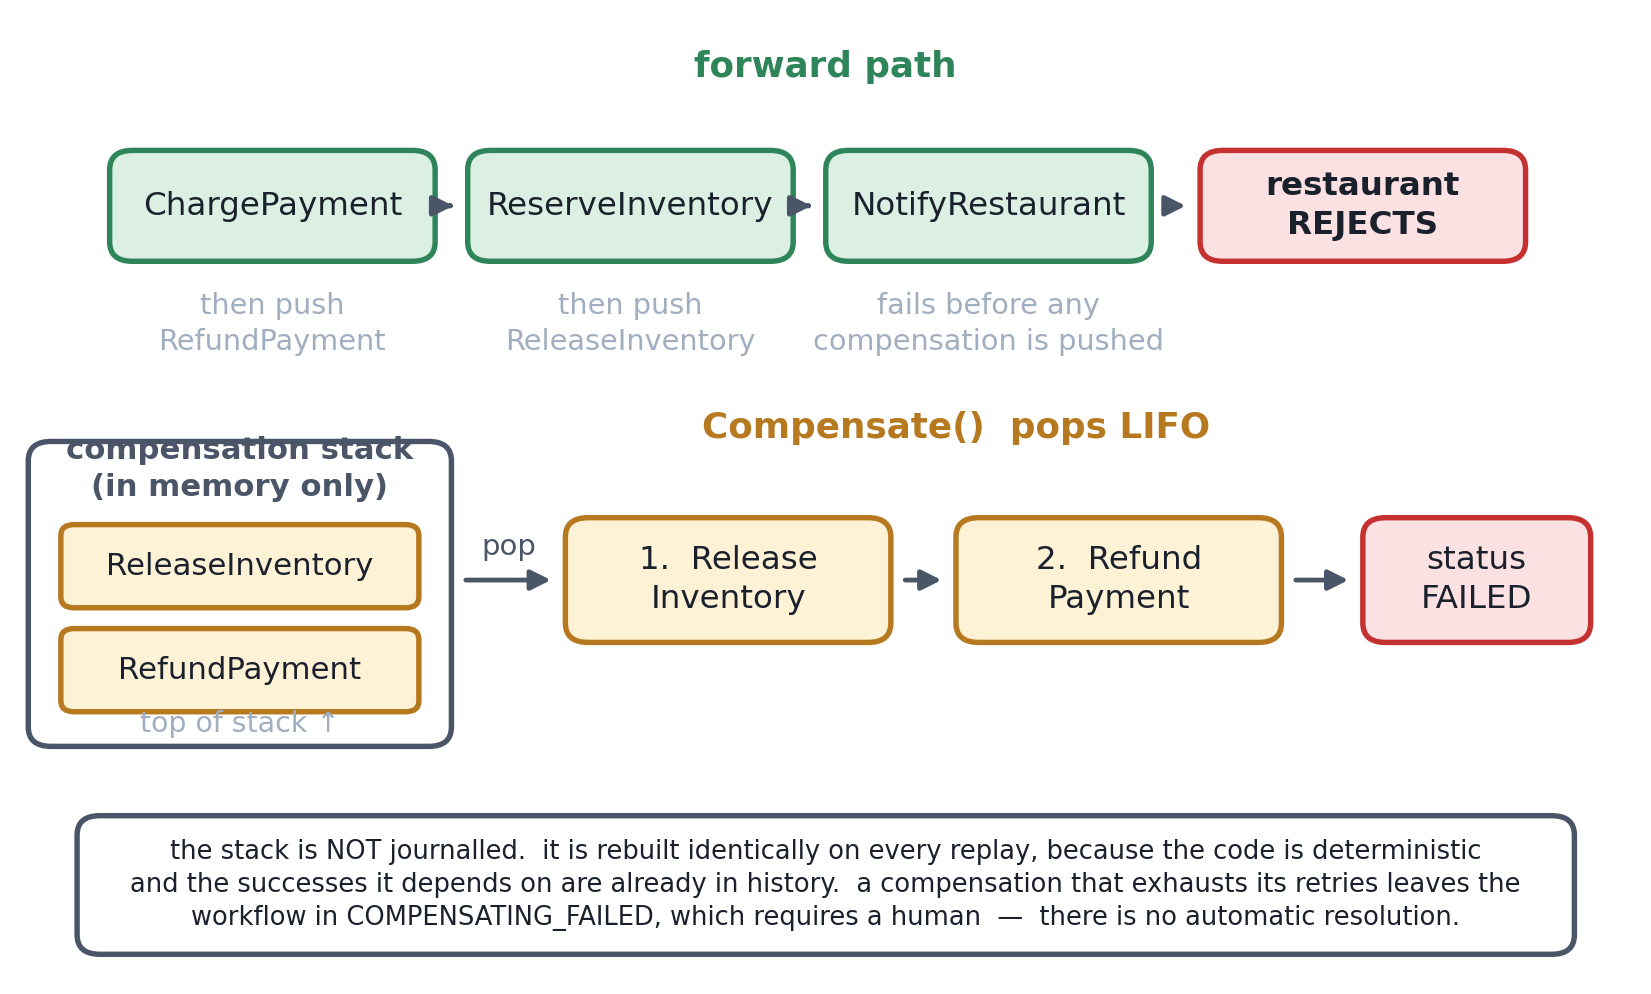
\includegraphics[width=\linewidth]{figures/fig_4_8_saga.png}
  \caption{Saga compensation. The stack exists only in memory and is rebuilt
    by replay; compensations run in reverse order as ordinary activities; and a
    compensation that exhausts its retries leaves the workflow in a terminal
    state requiring human intervention.}
  \label{fig:saga}
\end{figure}

Three hard cases are raised here rather than left to be discovered.

\textbf{A compensation can itself fail.} It retries with backoff like any
activity. If it exhausts its retries, the workflow enters
\cd{COMPENSATING\_FAILED} and requires human intervention (FR-13). There is no
automatic resolution, and the original saga formulation says as
much~\cite{sagas1987}. Surfacing the state in the administrative interface is
the correct response.

\textbf{Some steps cannot be compensated.} A sent email cannot be unsent. The
saga's guarantee is \emph{semantic} rollback --- a cancellation message ---
not \emph{physical} rollback.

\textbf{Sagas provide no isolation.} Between a step and its compensation,
other workflows can observe the intermediate state. Sagas are ACD rather than
ACID. Daraghmi et al.~\cite{daraghmi2022} attack exactly this gap with a quota
cache; this project accepts the limitation rather than solving it, and says
so.

\subsection{The Semantic Idempotency Decision Path}

This subsection specifies the research contribution of the project.

\subsubsection{The precise failure being addressed}

A framing correction is necessary first, because a loose statement of this
problem is easy to refute. When the \emph{engine} retries a scheduled
activity, the arguments are already frozen in the \cd{ActivityTaskScheduled}
event and are byte-identical on every attempt. Exact matching handles that
case completely. An engine-level retry is therefore \emph{never} the source of
a re-worded duplicate.

The real source is \textbf{agent re-planning}, and the sequence that produces
it is the one shown earlier in Fig.~\ref{fig:semanticgap}. A plan is
journalled; a tool call executes and books a flight; a second planning step
begins and the process crashes before that step's result is journalled. On
recovery, replay resolves the first plan and the tool call from history
without re-running them, but the second planning step genuinely re-executes.
At a non-zero sampling temperature it returns a different plan, which
re-issues the same intent in different words. The exact-match hash equals no
prior key, the action executes, and the flight is booked twice.

The claim is therefore stated narrowly and defensibly: \emph{agent
re-planning, whether triggered by a crash or by a tool failure, produces
semantically duplicate tool calls; the workflow's event history is the natural
place to detect them; and no durable execution engine looks there.}

\subsubsection{Where the verdict must be computed, and why}

The naive placement is inside the activity worker, immediately before the tool
is called. \textbf{That placement is wrong, and understanding why is the
strongest statement this design can make about itself.}

The similarity check is non-deterministic. It depends on an embedding model, a
floating-point threshold and a candidate set. Were the verdict computed inside
the activity worker, then on replay it would either be recomputed --- possibly
differently, causing history to diverge --- or skipped entirely, meaning the
workflow's decision would not be reproducible. Either outcome breaks the
governing principle of Section~4.1.1.

The correct placement follows directly: \textbf{the verdict is computed once,
on the workflow path, and journalled as an event.} It is the \cd{SideEffect}
pattern of Section~4.2.5 applied to a deduplication decision.
Fig.~\ref{fig:semdedup} shows both modes, and Listing~\ref{lst:semdedup} gives
them step by step.

\begin{figure}[htbp]
  \centering
  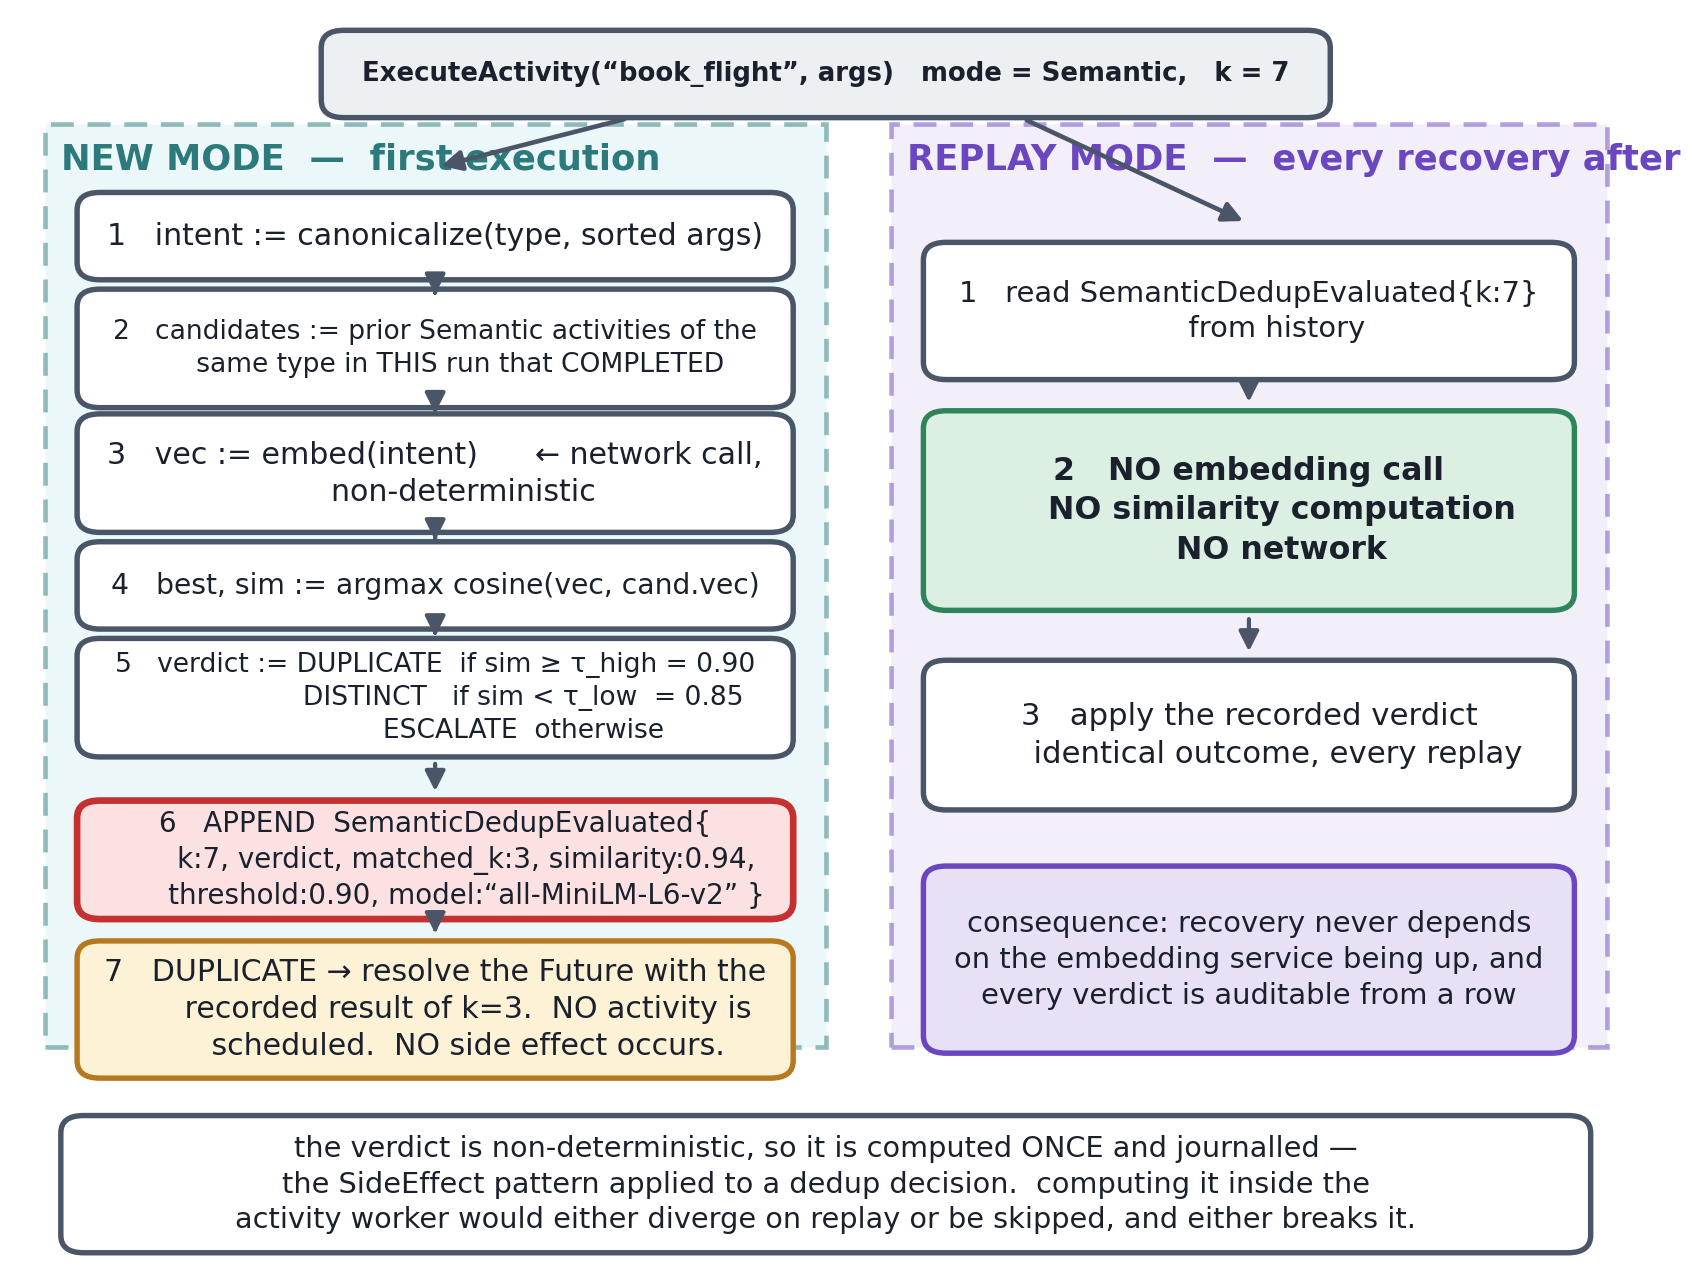
\includegraphics[width=\linewidth]{figures/fig_4_9_semantic_dedup.png}
  \caption{The semantic idempotency decision path. The non-deterministic
    verdict is computed once in new mode and journalled; every subsequent
    replay reads the recorded verdict and performs no embedding call, no
    similarity computation and no network access.}
  \label{fig:semdedup}
\end{figure}

\begin{lstlisting}[caption={The decision path in both modes. The asymmetry
  between them is the entire mechanism.}, label={lst:semdedup}]
ExecuteActivity("book_flight", args)   mode = Semantic,   at k = 7

NEW MODE:
  1. intent     := canonicalize("book_flight", sorted normalized args)
  2. candidates := prior Semantic activities of the SAME type in THIS
                   run's history that COMPLETED successfully
  3. vec        := embed(intent)             -- network, non-deterministic
  4. best, sim  := argmax cosine(vec, candidate.vec)
  5. verdict    := DUPLICATE  if sim >= tau_high (0.90)
                   DISTINCT   if sim <  tau_low  (0.85)
                   ESCALATE   otherwise
  6. APPEND  SemanticDedupEvaluated{ k:7, verdict:"DUPLICATE", matched_k:3,
             similarity:0.94, threshold:0.90, model:"all-MiniLM-L6-v2" }
  7. DUPLICATE -> resolve the Future with the recorded result of k=3.
                  NO activity is scheduled.  NO side effect occurs.
     DISTINCT  -> emit ScheduleActivity as normal.
     ESCALATE  -> emit a human-approval signal wait, or execute (configurable).

REPLAY MODE:
  1. Read SemanticDedupEvaluated{k:7} from history.
  2. NO embedding call.  NO similarity computation.  NO network.
  3. Apply the recorded verdict.  Identical outcome, every replay, forever.
\end{lstlisting}

Three consequences follow and are worth stating explicitly.

\textbf{Replay is fast and offline.} No embedding service is needed in order
to recover a workflow. If the embedding provider is unavailable, in-flight
workflows still recover normally. A design that called the model on every
replay would have coupled recovery availability to a third-party API, which is
the kind of dependency this project exists to avoid. This satisfies constraint
C-4.

\textbf{The verdict is auditable.} The stored event carries the similarity,
the threshold, the matched predecessor and the model identifier. When somebody
asks why a particular flight was never booked, the answer is a row rather than
a reconstruction. For a mechanism empowered to suppress real-world actions,
that audit trail is not a convenience; it is what makes the feature deployable
(NFR-10, FR-15).

\textbf{It composes with the existing determinism story} rather than fighting
it, because it is an instance of a mechanism the engine already had.

\subsubsection{Storage and the candidate set}

Intents are stored in a dedicated table keyed by shard, workflow, run and
scheduled sequence, carrying the canonicalised intent text and a
384-dimensional embedding vector held in a \cd{VECTOR(384)} column.

Candidate sets are per-workflow-run and small --- tens of rows. Brute-force
cosine similarity over a set that size takes microseconds, and no approximate
nearest-neighbour index is required. This is worth stating explicitly, because
it pre-empts the obvious scaling objection: the search is bounded by the
length of one workflow's history, not by the size of a global corpus. That is
a genuine architectural advantage over semantic caching
systems~\cite{gptcache2023}, which must search a corpus shared by all users.

The construction of the intent text matters more than the choice of model. The
canonical form is the activity type followed by its sorted, normalised
arguments. For an activity such as \cd{search\_flights} whose argument is
itself natural language, this embeds meaningfully. For an activity such as
\cd{charge\_payment} whose argument is an amount, it does not --- which is
precisely why the idempotency mode is opt-in per activity and defaults to
exact matching.

\subsubsection{Failure modes, stated first}

\begin{table}[htbp]
  \centering
  \caption{Failure modes of the semantic comparator. The asymmetry between
    them is the design's central constraint.}
  \label{tab:semfail}
  \small
  \begin{tabular}{@{}p{0.7in}p{1.38in}p{1.02in}p{1.58in}@{}}
    \toprule
    & \textbf{Meaning} & \textbf{Cost} & \textbf{Mitigation} \\
    \midrule
    \textbf{False positive} &
      Two genuinely different calls are judged duplicate, so a real action is
      silently skipped &
      \textbf{Severe and asymmetric.} A flight the user wanted is never booked,
      and nothing reports an error &
      Opt-in per activity; high $\tau$; escalation band; every verdict
      journalled and visible in the administrative panel \\
    \textbf{False negative} &
      A true duplicate is not caught and executes twice &
      Equal to the exact-match baseline. No regression & None required \\
    \bottomrule
  \end{tabular}
\end{table}

The asymmetry in Table~\ref{tab:semfail} is the honest core of this
contribution and is presented as a designed-for constraint rather than left to
be discovered: \textbf{the mechanism is strictly better than the baseline on
false negatives and strictly worse on false positives, and it is therefore
opt-in, conservatively thresholded and fully audited.} Claiming the mechanism
is free is what would invite the design to be picked apart.

The two-threshold structure, with an escalation band between $\tau_{low}$ and
$\tau_{high}$, is taken from work on calibration in semantic
caching~\cite{calibration2026}, which shows that a single threshold forces a
binary decision at exactly the point where the model is least confident. The
difficulty of calibrating such a threshold at all is not a shortcoming unique
to this project: vCache~\cite{vcache2026} reports the same finding across
approximately 45{,}000 examples, with problematic cut-offs falling in the same
range this design uses.

Finally, the relationship to the closest competing work bears restating. Robust
Agent Compensation~\cite{rac2026} undoes an agent's actions after a failure is
detected. This mechanism prevents the duplicate from executing. A duplicate
that succeeds raises no failure and therefore triggers no compensation, which
is precisely the case this design catches and RAC cannot.

\subsection{Node Runtime Composition}

The design concludes with what actually runs on a machine. One Go binary, one
process per node, with the goroutine structure shown in
Fig.~\ref{fig:runtime}: an HTTP server, a lease manager, a metrics collector,
and --- for each shard the node currently owns --- one timer scanner, four
workflow workers and eight activity workers.

\begin{figure}[htbp]
  \centering
  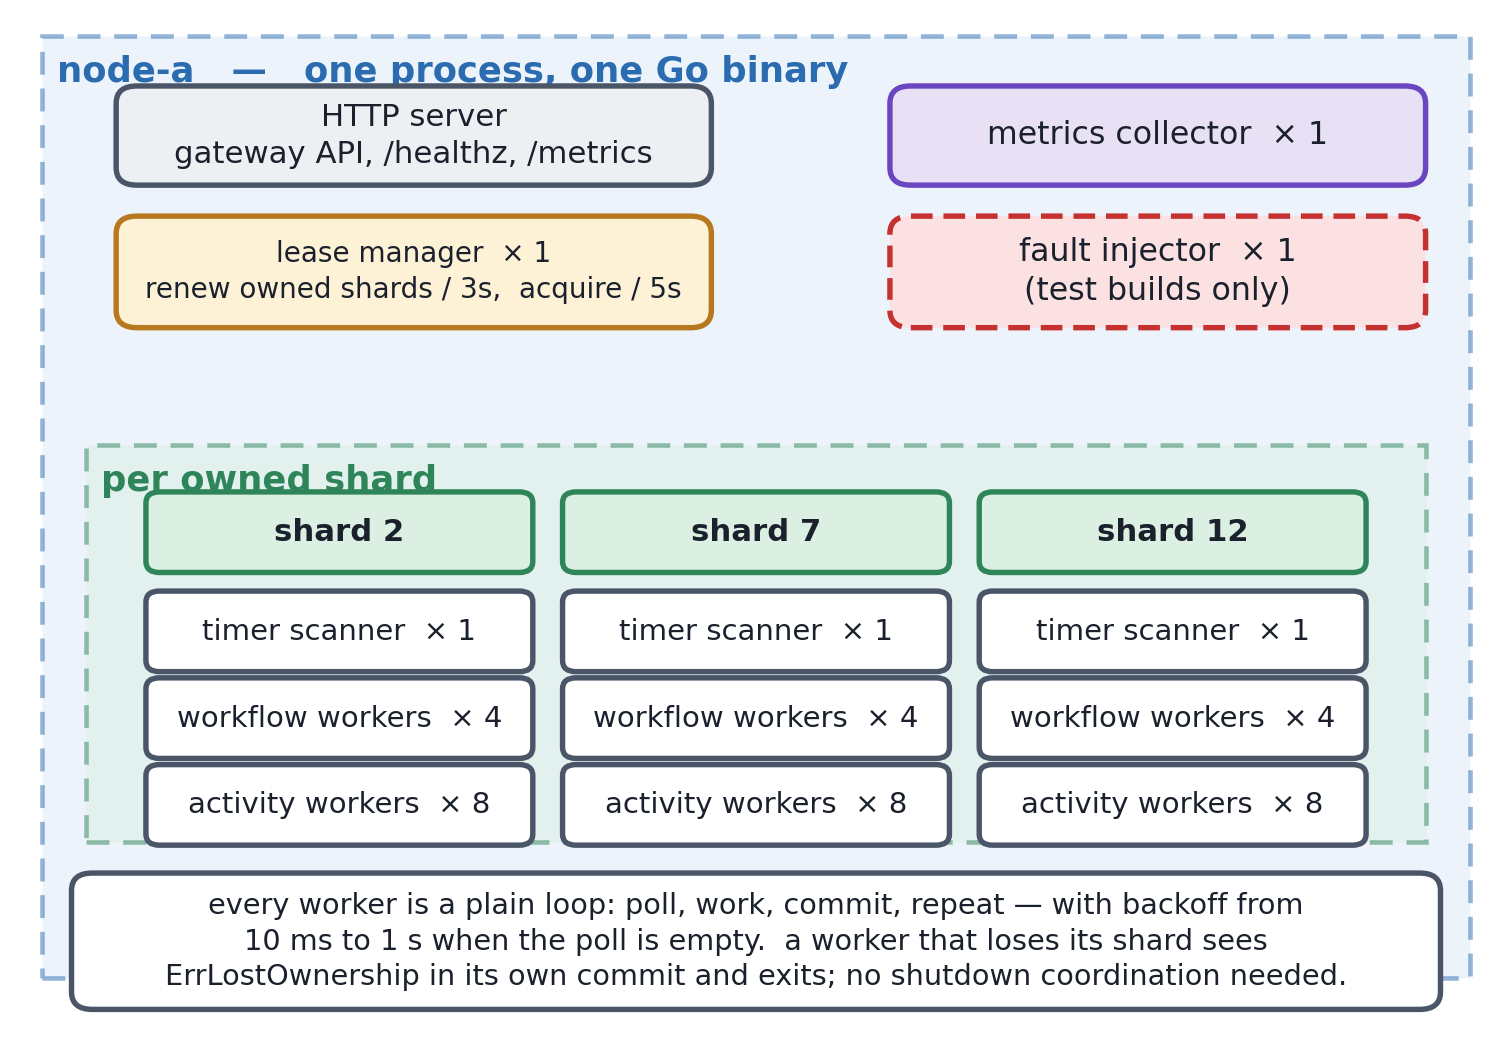
\includegraphics[width=\linewidth]{figures/fig_4_10_node_runtime.png}
  \caption{The goroutine composition of one node. Worker counts are per owned
    shard, so a node's concurrency scales with the number of shards it owns
    rather than with cluster size.}
  \label{fig:runtime}
\end{figure}

Each worker goroutine is a plain loop: poll, do the work, commit, repeat, with
exponential backoff from ten milliseconds to one second when a poll returns
nothing, so that an idle cluster does not saturate the database.

The shutdown path deserves a closing observation, because it demonstrates the
economy the fencing design buys. Every worker verifies the fencing token
inside its own commit. If a shard is lost while work is in flight, its workers
discover this when their own transaction fails, abandon it and exit.
\textbf{No coordination is required to shut them down, and no supervisor needs
to notify them --- the database tells them.} A mechanism designed for
correctness under split-brain turns out to supply orderly shutdown as a side
effect, which is a reasonable indication that the abstraction was drawn in the
right place.

\begin{table}[htbp]
  \centering
  \caption{Runtime configuration parameters and their defaults}
  \label{tab:config}
  \small
  \begin{tabular}{@{}p{1.28in}p{0.6in}p{2.5in}@{}}
    \toprule
    \textbf{Parameter} & \textbf{Default} & \textbf{Meaning} \\
    \midrule
    \cd{ShardCount} & 16 &
      Fixed partition count; see Table~\ref{tab:ringparams} \\
    \cd{LeaseTTL} & 10\,s & Lease duration, bounding failover time \\
    \cd{LeaseRenew} & 3\,s & Renewal interval, giving three attempts per TTL \\
    \cd{TaskLock} & 30\,s &
      Visibility timeout on a claimed task; must exceed the longest expected
      activity \\
    \cd{WorkflowWorkers} & 4 & Workflow worker goroutines per owned shard \\
    \cd{ActivityWorkers} & 8 &
      Activity worker goroutines per owned shard; higher than the workflow
      count because activities block on external I/O \\
    \cd{SyncCommit} & true &
      Synchronous replication, trading throughput for a zero loss window \\
    \cd{TauHigh} & 0.90 & Similarity at or above which a call is a duplicate \\
    \cd{TauLow} & 0.85 &
      Similarity below which a call is distinct; the band between the two
      escalates \\
    \bottomrule
  \end{tabular}
\end{table}

The design presented in this chapter is complete to the level at which it can
be implemented. Chapter~5 describes that implementation, Chapter~6 the testing
strategy, and Chapter~7 the measured results of running the engine under
deliberately induced failure.

